\section{Empirical Measurements}
\label{section:Empirical_measurements}

% Begin this section with a brief introduction about what empirical measurements are, why they are necessary, and what they aim to determine or reveal in the context of stray fields in the PS

Empirical measurements constitute the fundamental foundation to validate and improve simulation models, specifically in examining the initial conditions of the beam at the exit of the PS. These assessments are conducted through quadrupole scans at the East Dump.

\begin{figure}[htbp]
\centering
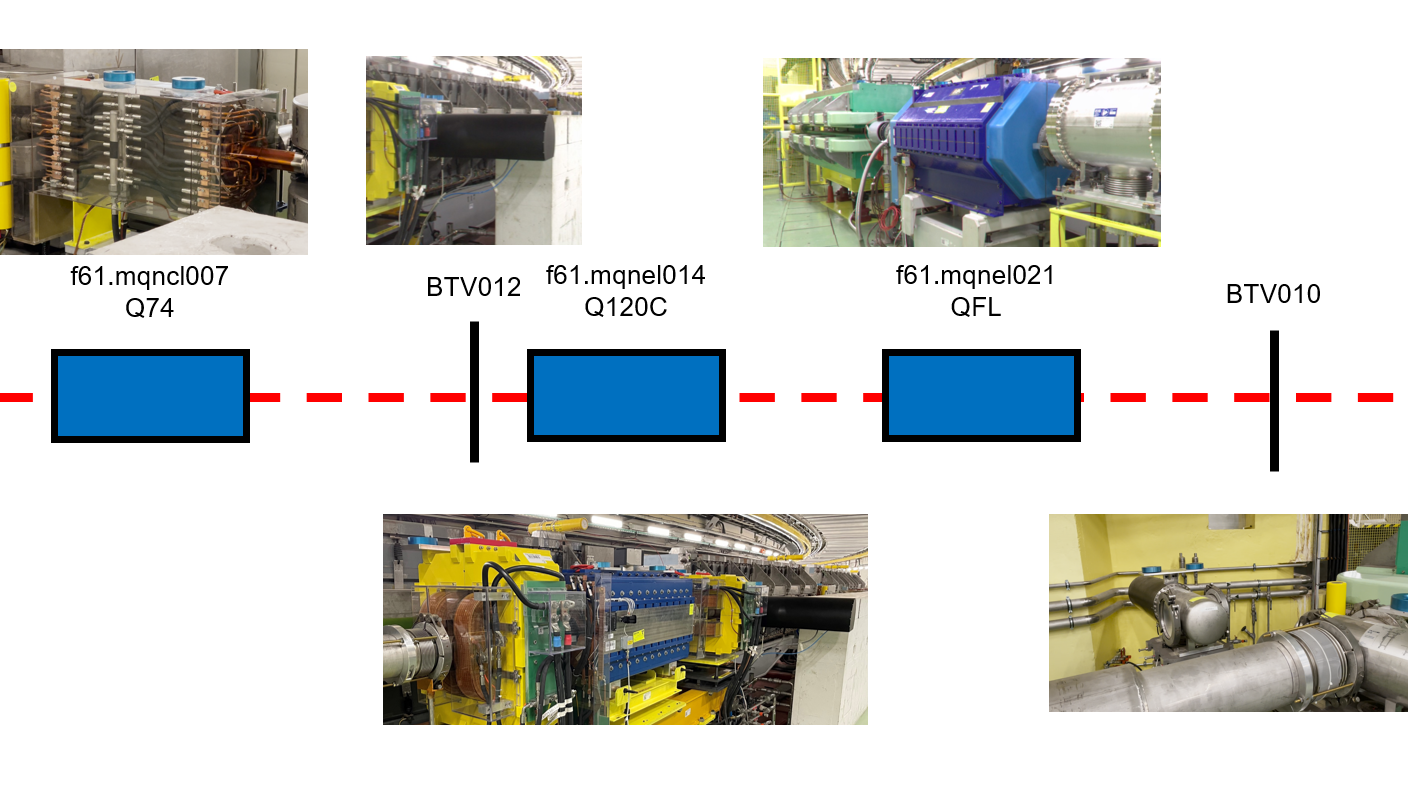
\includegraphics[width=\linewidth]{03_Empirical_Measurements/images/East_dump_line.png}
\caption{Diagram of the East Dump Line which comprises three quadrupoles and a bending magnet that directs the beam to the dump (F6D.TDE018). Two BTVs (BTV012 and BTV010) are used for beam measurements.}
\label{fig:East_dump_line}
\end{figure}

Situated within the East Area complex is a short line, designed for extraction studies, which leads to a dump aptly named the East Dump Line, see Fig. \ref{fig:East_dump_line}. The East Dump Line is ideally suited for quadrupole scans due to its configuration of three upstream quadrupoles used to modify the optics. Additionally, it houses two Beam-TV (BTVs) (F61.BTV012 and F61D.BTV010) for beam observation. Notably, the line can be used for parallel Machine Development (MD) without disrupting operational beams directed at the experimental targets in the East Area. Each BTV employs a fluorescent screen which can be remotely inserted into the beam line during measurements, see Fig. \ref{fig:btv_diagram}. The interaction of the particles with the material produces light which a camera system subsequently captures through a viewport. The image collected corresponds to the beam "footprint" on the screen, serving a valuable tool for beam observation, steering or measurement. The insertion of the screen has the downside of significantly degrading the beams properties, such as the beam size, through material interaction and care must be taken when used in parallel of other beams. This issue doesn't not concern the East Dump line as BTV010 is placed in front of the East Dump which can be used exclusively for extraction and optics MDs.

\begin{figure}[htbp]
\centering
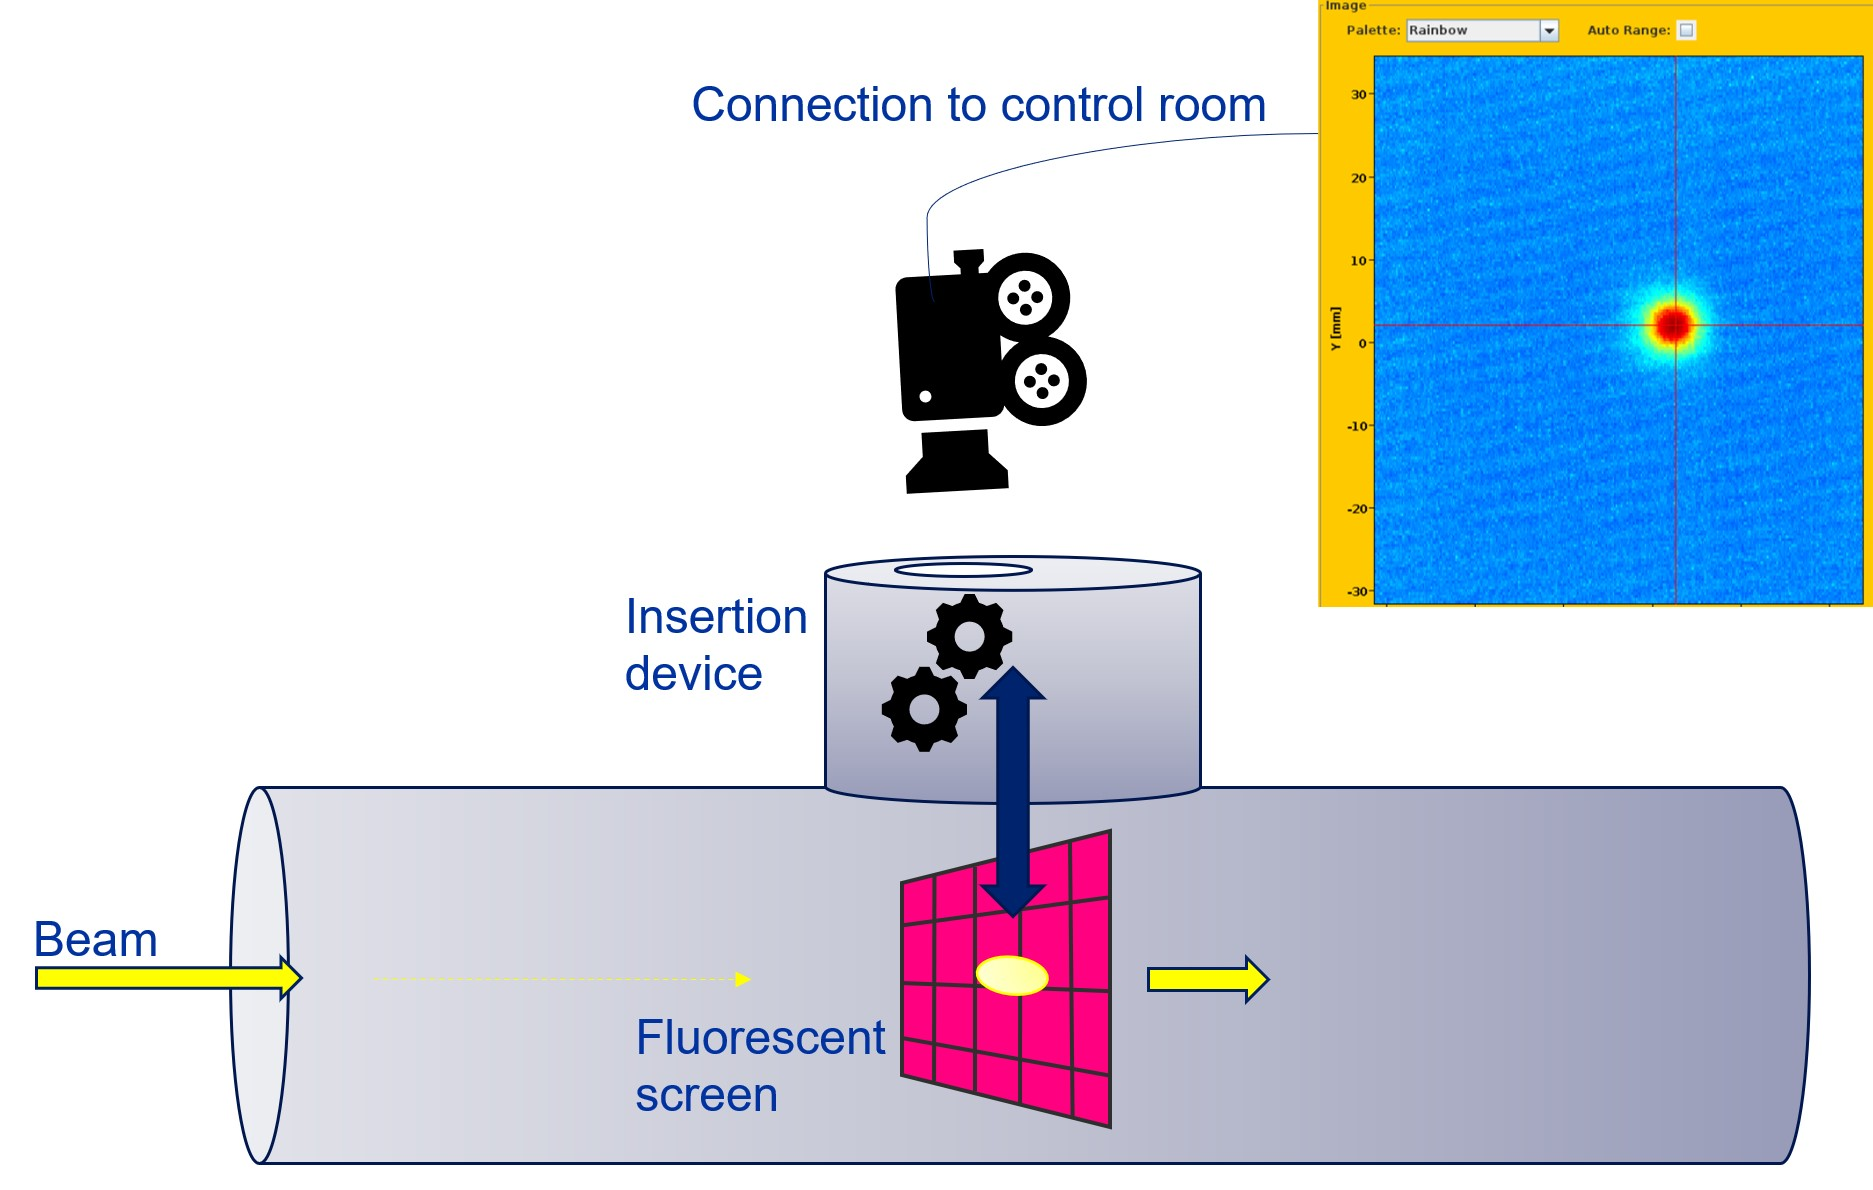
\includegraphics[width=0.7\linewidth]{03_Empirical_Measurements/images/BTV_diagram.jpg}
\caption{BTV Diagram}
\label{fig:btv_diagram}
\end{figure}

\subsection{Quadrupole scan}

% Describe the process and the purpose of the quadrupole scan. You should discuss:
% The objective of the scan.
% The setup: What equipment is used? How is the experiment arranged?
% The process: How is the scan conducted?
% The results: What data was collected? What are the key findings from the scan?

A quadrupole scan are used to measure beam parameters and involves adjusting the strength of a quadrupole, and subsequently observing the variations in the beam size ($\sigma$) and beam position (centroid) across both planes using an instrument located downstream of the quadrupole being modified, see Fig. \ref{fig:quad_scan_example}. The objective of this scan is to finely tune the simulation tool MAD-X \cite{noauthor_mad_nodate} to enable the prediction of beam sizes through a model that has been adjusted according to these measurements. To achieve this, the initial parameters of the MAD-X model are aligned with the observed measurements as accurately as possible. It is generally advantageous to find the minimum and maximum values of the beam size at the instrument's location, which facilitates the reconstruction of the rematching of the initial conditions. The parameter-matching process is conducted in Python, utilizing either the Scipy or the Py-BOBYQA library \cite{cartis_improving_2019, cartis_escaping_2022}.

\begin{figure}[htbp]
\centering
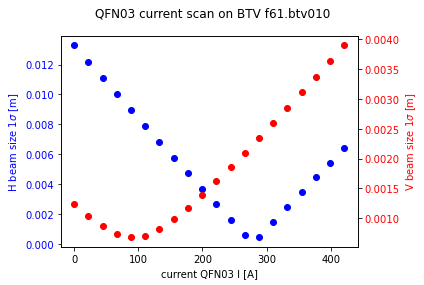
\includegraphics[width=0.5\linewidth]{03_Empirical_Measurements/images/quadrupole_scan_east_dump.png}
\caption{Example of a quadrupole scan with minimums in both planes measured on the East Dump BTV.}
\label{fig:quad_scan_example}
\end{figure}

A quadrupole scan can also serve as a tool to inform about the relative offset between the beam and the quadrupole's center. Operationally, there is a high likelihood that the beam is not perfectly centered within a quadrupole. In such instances, any alteration in the quadrupole's strength will not only affect the beam size or the optics, which is the expected primary effect, but will also induce a dipole moment. This, in turn, will shift the centroid of the beam. In simpler terms, if a scan in current/strength of a quadrupole is conducted, and there is a misalignment in either the beam or the quadrupole, it will result in the beam being steered. Figure \ref{fig:misaligned_quadrupole} provides a simulation of the East Dump Line with the first quadrupole misaligned by a positive offset of 0.01 m in the x direction (to the left in the beam's path). The color-coded traces illustrate the different paths that the particle will follow as the quadrupole's strength is adjusted. This however cannot distinguish between the quadrupole being offset and the beam being mis-steered.
\\

\begin{figure}[htbp]
\centering
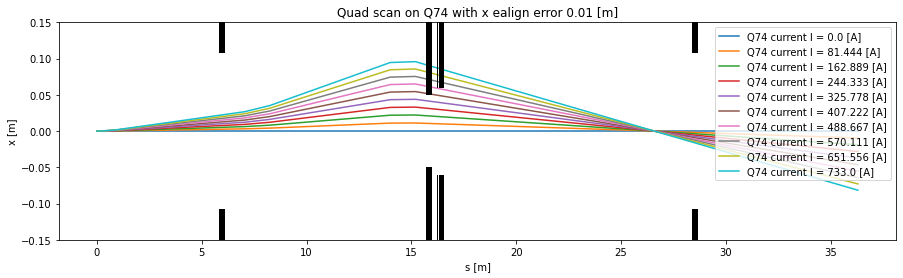
\includegraphics[width=\linewidth]{03_Empirical_Measurements/images/misaligned_quadrupole.png}
\caption{MAD-X simulation of a quadrupole being misplaced and impact of quadrupole strength variation.}
\label{fig:misaligned_quadrupole}
\end{figure}

Figure \ref{fig:misaligned_quadrupole_2} displays the displacement of the centroid as a function of current, with the quadrupole Q74 being misaligned by different values. This plot can help understand in which direction the beam will move and by how much if not properly centered. Additionally and important to note an offset in the beam position will not modify the beam size.
\\

\begin{figure}[htbp]
\centering
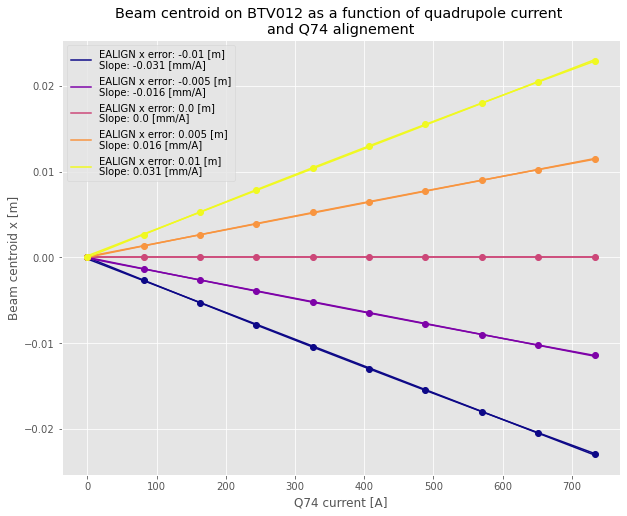
\includegraphics[width=0.7\linewidth]{03_Empirical_Measurements/images/misaligned_quadrupole_2.png}
\caption{Misaligned quadrupole simulation}
\label{fig:misaligned_quadrupole_2}
\end{figure}

CERN frameworks facilitate the adjustment of current in specific quadrupoles through Python, utilizing a library known as PyJapc \cite{noauthor_scripting-tools_2023}. A suite of quadrupole scan scripts, employed in this note, can be accessed via the following GitLab repository:  \href{https://gitlab.cern.ch/eljohnso/quad-scan-east}{gitlab.cern.ch/eljohnso/quad-scan-east}. Referring to the quadrupole beam offset just discussed, a simple script called \href{https://gitlab.cern.ch/eljohnso/quad-scan-east/-/blob/master/check_centered_in_quad.py}{check\_centered\_in\_quad.py} scans three currents in a specific quadrupole and looks at the mean position of the gaussian fit on a BTV. It continuously takes the last three centroid measurement ($\mu$) which can be used for informed beam steering.

\subsubsection{East Area BTV}
BTVs are one of the instrumentation used in this report and some explanation on how they operate is required. Specific to the extraction in the East Area is that during a slow extraction ($\sim$ \SI{400}{ms}) the BTVs are capable of multiple acquisitions. This can be used to take the multiple beam size measurements during the spill and observe any difference in beam position or trend such as a sweep. As it turns out, the beam size changes during the spill which means the optics during extraction isn't constant. This is why when finding initial parameters or rematching a single acquisition from the BTV was chosen (in the middle of the spill) to best represent the beam. Most of the time the fourth acquisition was chosen as it is once the beam is stabilised (after the Figure-of-eight Loop's (F8L) eddy currents). The East Area BTV system is comprised of two crates: cfv-157-btv1, which includes PR57, F62, F61, and F61D, and cfv-157-btv2, which includes all T8 BTVs. There are three crucial parameters that can be changed in these two crates: PE2X.SACQ-EMTV2 (\textbf{S}tart \textbf{ACQ}uisition), PE2X.ACQ-EMTV2 (delay between \textbf{ACQ}uisition), and PE2X.EACQ-EMTV2 (\textbf{E}nd \textbf{ACQ}uisition).

\begin{enumerate}
    \item The PE2X.SACQ-EMTV2 parameter is adjustable, with a caveat that the initial event is lost due to the offset of the initiation timing. Presently, the acquisition begins 900 ms prior 1030 ms extraction start, plus an additional 720 ms delay, culminating in a start time at 850 ms. The first acquisition occurs at 950 ms (850 plus a 100 ms delay) with subsequent acquisitions every 100 ms, see Fig. \ref{fig:btv_timing}. Previously, the start timing for the BTVs began at PE2X-W20, a 20 ms pre-extraction warning. However, BI made modifications such that the timing now starts at PE2X.F900-CT, a 900 ms forewarning before extraction. The starting event can be verified through LTIM cfv-157-btv2.LTIM and PE2X.SACQ-EMTV2/LoadEvent.
    \item The PE2X.ACQ-EMTV2 parameter determines the interval between each image acquisition. By setting this parameter to zero and scrutinizing the acqTimeInCycle, it is possible to compute the time required for each acquisition which is $\sim$ 70 ms.
    \item The PE2X.EACQ-EMTV2 parameter signals the end of the acquisition period, which begins at PX.ELFT-CT, marking the \textbf{E}nd of the flat top (\textbf{FT}) cycle plus an additional 200 ms. This parameter is configured in such a way as to ensure that the seven acquisition instances occur within each cycle (lasting 2400 ms).
\end{enumerate}

\begin{figure}[H]
\centering
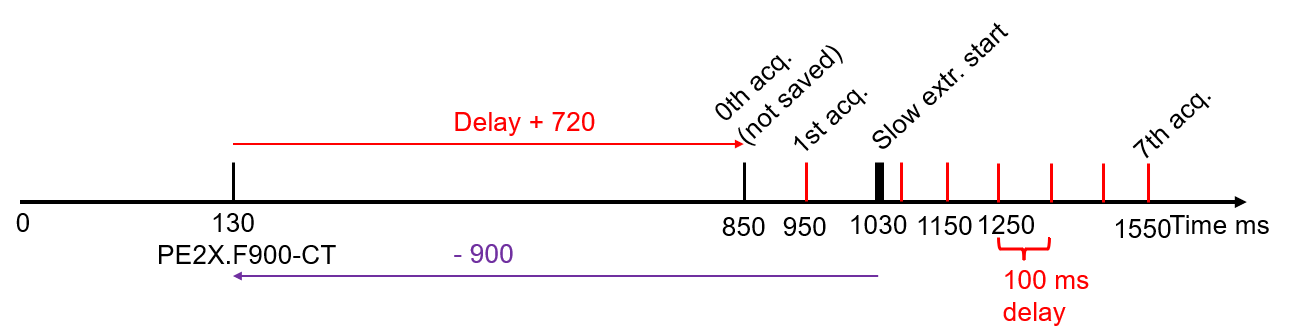
\includegraphics[width=1.0\linewidth]{03_Empirical_Measurements/images/btv_timing.png}
\caption{East Area BTV timing}
\label{fig:btv_timing}
\end{figure}


The BTVs operate asynchronously, leading to a jitter of 20 ms between each frame, see Fig. \ref{fig:btv_jitter}. However, with the imposed delay, we plan for an empty frame at the beginning, which can be used for background noise removal. It is possible to install a hardware trigger to remove the jitter as it is done in the other lines but this is currently not installed in the East Area.

\begin{figure}[ht]
\centering
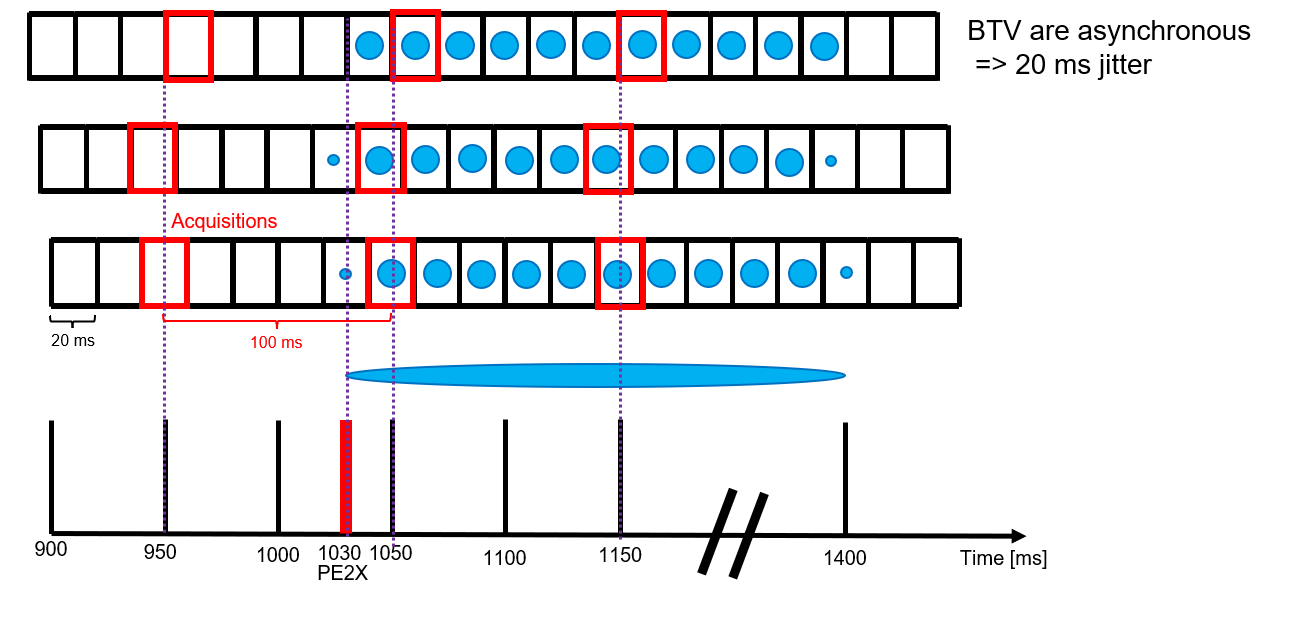
\includegraphics[width=1.0\linewidth]{03_Empirical_Measurements/images/btv_jitter.png}
\caption{BTV jitter}
\label{fig:btv_jitter}
\end{figure}

The fastest achievable full-resolution acquisition occurs with a delay of 90 ms. Further reduction of the delay yields inconsistent timing, with substantial skips occurring below 60 ms. Acquisition speeds can be increased by reducing the size of the frame (number of pixels), which reduces data flow. However, a bottleneck persists. Lowering the resolution further may still result in inconsistent timing, but if the acquisition time in cycle is saved, it may still be useful for measurements that require a higher repetition rate.

\subsubsection{Filter wheels}

In the East Area, filter wheels have been installed in front of the BTVs to regulate the light intensity reaching these devices, thereby preventing saturation. Saturation of the detector greatly diminishes the accuracy of the beam size measurement and should be avoided. Four filter settings are available on the filter wheel: none, OD1, OD2, OD3. Each filter reduces the quantity of light attaining the BTV by an order of magnitude. Specifically, OD1 allows 10\% of the light to pass, while OD2 and OD3 permit 1\% and 0.1\% respectively.
\\

During the nominal slow extraction at an intensity of $59.7\cdot10^{10}$ particles per spill, the BTVs are saturated with the OD2 filter but not with the OD3 filter. It is pertinent to note that the saturation level will depend on the optics and diligence is required during a quadrupole scan to monitor for both variation in beam size and saturation. If significant changes in beam size are made, the use of multiple filters may become necessary. A straightforward saturation alarm mechanism can be implemented by counting the number of pixels at maximum value. As well as removing saturation, filters can be leveraged to to suppress beam remanence, which may otherwise lead to inflated beam size measurement during a spill in the presence of beam movement.
\\

Figures \ref{fig:sigmaH} and \ref{fig:sigmaV} present the beam size against the acquisition number (analogous to time along the spill) in the horizontal and vertical planes respectively, with each filter setting. Each set comprises 25 measurements, with the mean indicated by a dot. These figures reveal substantial differences in beam size between filters due to saturation and remanence, as well as changes in beam size throughout the spill due to a (unwanted) non-constant optic.
\\

\begin{figure}[htbp]
    \centering
    \begin{subfigure}[b]{0.49\textwidth}
        \centering
        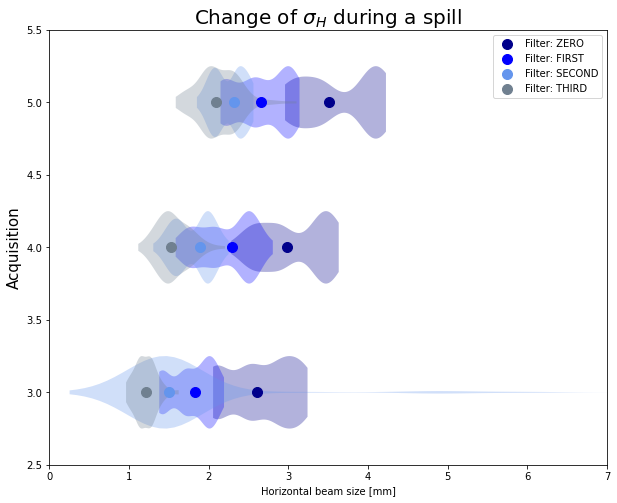
\includegraphics[width=\textwidth]{03_Empirical_Measurements/images/sigmaH.png}
        \caption{Horizontal beam size}
        \label{fig:sigmaH}
    \end{subfigure}
    \hfill
    \begin{subfigure}[b]{0.49\textwidth}
        \centering
        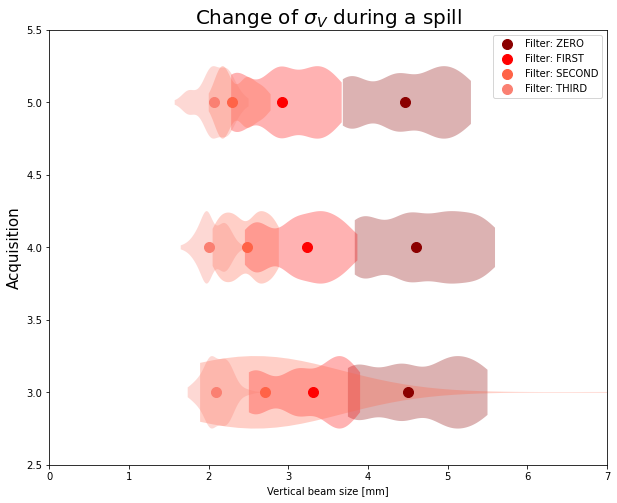
\includegraphics[width=\textwidth]{03_Empirical_Measurements/images/sigmaV.png}
        \caption{Horizontal beam size}
        \label{fig:sigmaV}
    \end{subfigure}
    \caption{Comparison of beam size during a spill average of 25 acquisitions.}
    \label{fig:filter_sigma}
\end{figure}

Figures \ref{fig:centroidH} and \ref{fig:centroidV} display the centroid in both planes across the different filters. Here, the filters are not critical for obtaining accurate beam position measurements, as expected. An additional relevant observation is that variations in intensity, either an increase or a decrease, can mitigate BTV saturation without influencing the beam size. This could be beneficial under certain experimental conditions.
\\

\begin{figure}[htbp]
    \centering
    \begin{subfigure}[b]{0.49\textwidth}
        \centering
        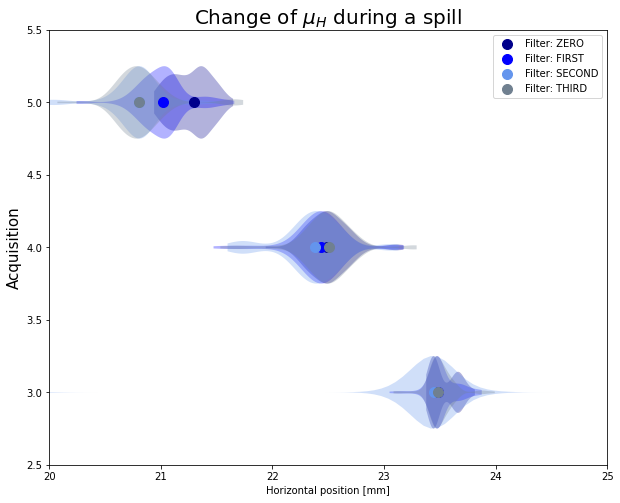
\includegraphics[width=\textwidth]{03_Empirical_Measurements/images/muH.png}
        \caption{Horizontal centroid}
        \label{fig:centroidH}
    \end{subfigure}
    \hfill
    \begin{subfigure}[b]{0.49\textwidth}
        \centering
        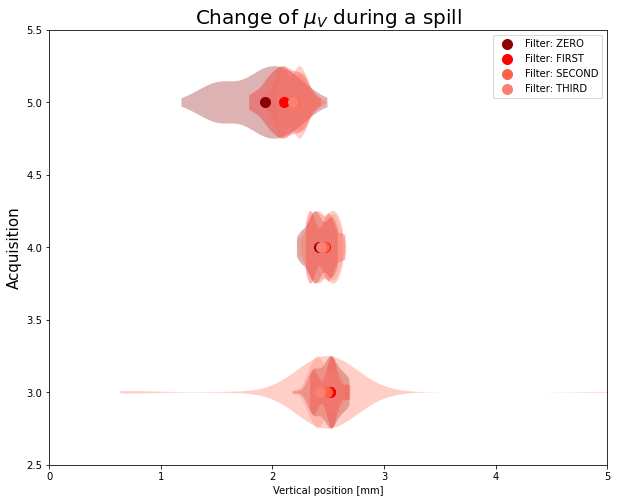
\includegraphics[width=\textwidth]{03_Empirical_Measurements/images/muV.png}
        \caption{Horizontal centroid}
        \label{fig:centroidV}
    \end{subfigure}
    \caption{Comparison of beam centroid during a spill average of 25 acquisitions.}
    \label{fig:filter_centroid}
\end{figure}

Accurate measurements of beam size, whether obtained through the use of filter wheels or alternative methods, are indispensable for precise determination of initial beam conditions. Previous use of saturated beam size data for MAD-X reconstruction has been found to yield inaccurate initial beam parameters. Therefore, ensuring the accuracy of beam size measurements is critical in for reliable beam characterization.
\\

\subsubsection{Image Processing Techniques}

To achieve precise beam size measurements using the BTVs, it is essential to apply image processing methods, given the inherent noise present in the raw image. The initial step involves processing the raw image through a sequence of a median filter and a Gaussian filter, which smooths neighboring pixels\footnote{Various filters such as bicubic interpolation and singular applications of either the median or Gaussian filter have been tested. However, for the present application, a sequential combination of the median filter followed by a Gaussian filter seems to be the most suitable.} and remove noise. This filtering step is succeeded by an initial Gaussian fit, used to estimate the beam center. The estimated beam size is then employed to create an elliptical mask, see Fig. \ref{fig:elliptical_mask}, facilitating the exclusion of regions far from the beam. Subsequently, a second Gaussian fit provides the final beam size measurement. Figure \ref{fig:image_processing} illustrates the enhancement in signal quality upon conducting these successive image processing steps.

\begin{figure}[htbp]
\centering
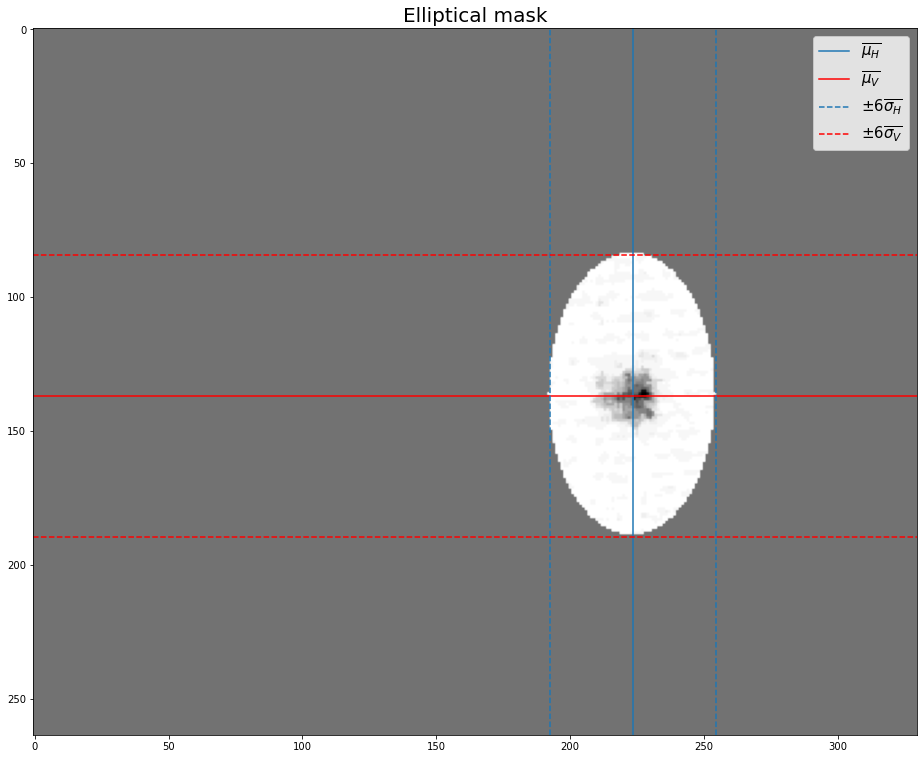
\includegraphics[width=0.7\textwidth]{03_Empirical_Measurements/images/elliptical_mask.png}
\caption{Elliptical mask applied to the processed BTV image, centered by using an initial gaussian fit with a multiple of $\sigma$ used for the dimension of the ellipse axis.}
\label{fig:elliptical_mask}
\end{figure}

\begin{figure}[htbp]
\centering
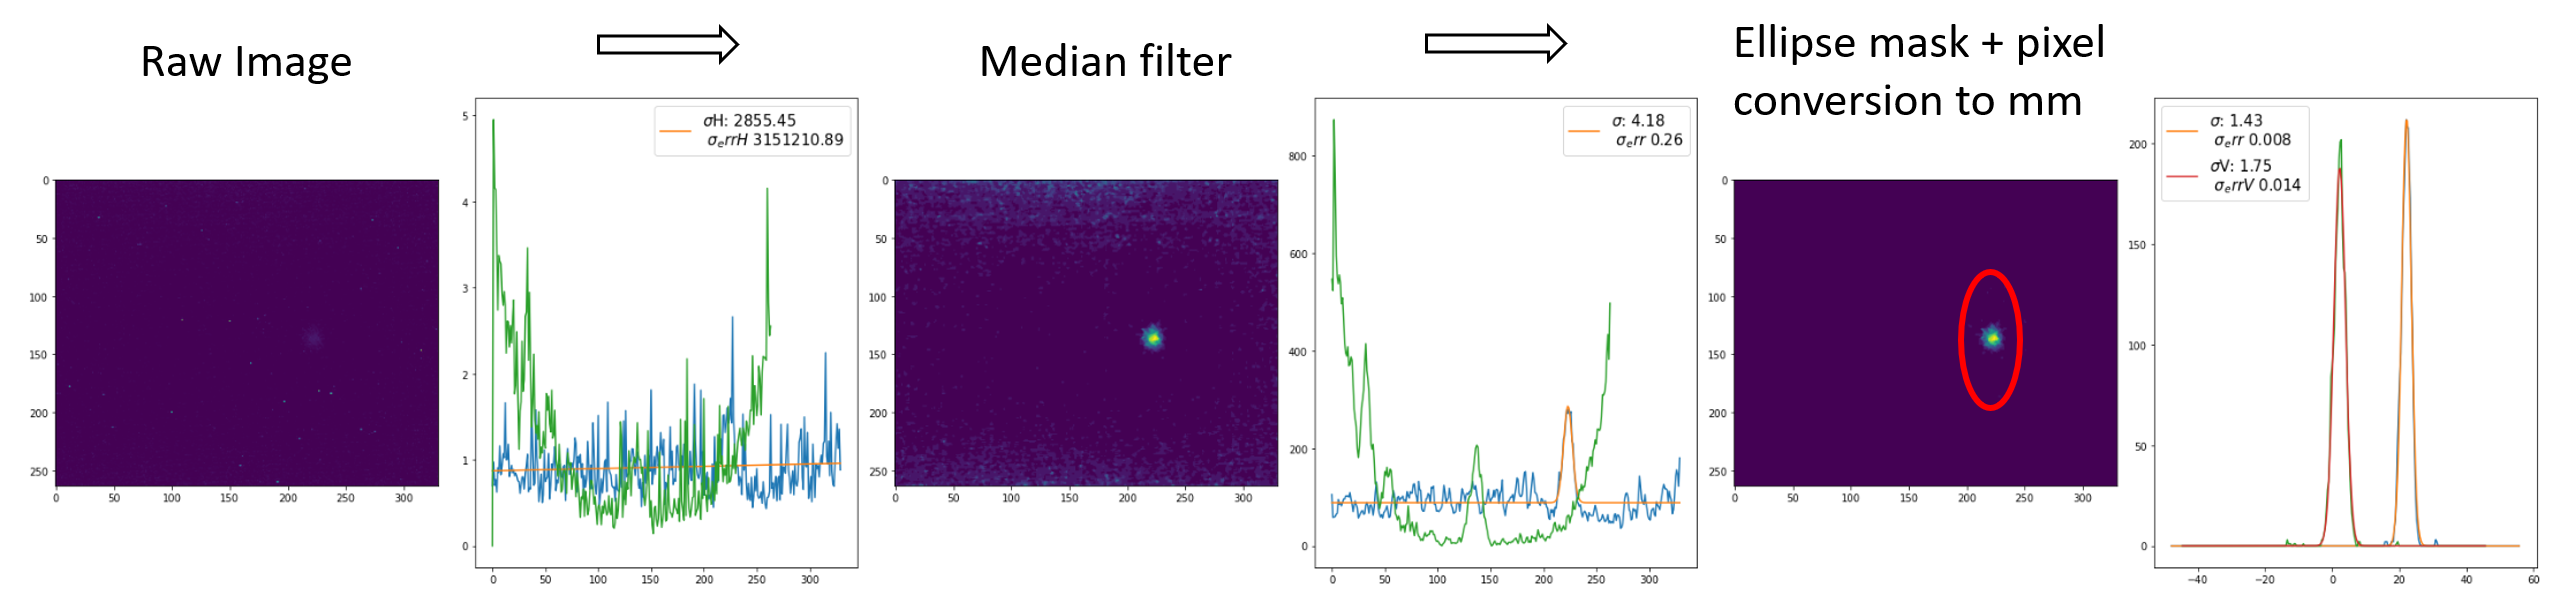
\includegraphics[width=\textwidth]{03_Empirical_Measurements/images/image_processing.png}
\caption{Illustration of signal quality improvement after consecutive image processing steps.}
\label{fig:image_processing}
\end{figure}

\subsubsection{Additional information on beam size measurement}

A few lessons are worth sharing to correctly reconstruct the initial parameters. In particular, one should carefully select the acquisition frame from the BTV so as to have a constant beam size. If it's at the edge of the spill, the beam might be cut because of the jitter in the acquisition. It is thus best to use an acquisition in the middle of the spill. Furthermore, the installation of filter wheels on the BTV is of invaluable to the reconstruction. Without filters, the fluorescent screen would saturate at high intensity which would give erroneous beam size measurements. Careful selection of the measurements from the quadrupole scan should be made. Combination of quadrupole at high and low strength might significantly alter the beam which could then scrap the apertures. Such measurement should be discarded. In general regions close to the minimum and maximum of the parabolas are sufficient. To speed up the optimisation algorithm an efficient way to prepare the measurement is to create a single data frame regrouping the parsed data with columns containing the quadrupole strength (K1s) and horizontal and vertical beam size.


\subsection{Transfer line initial condition reconstruction}

% This subsection should focus on how you identified the initial parameters for your study. Include the following points:
% A description of the parameters and their significance.
% The method used to determine these initial parameters.
% Any challenges faced and how you overcame them.
% The final list of initial parameters.

\subsection{Methodology}
The method to find the initial conditions of a transfer line using empirical measurements will now be described. First a set of quadrupole scan is collected by varying the strength (K1s) of a single or a combination of quadrupoles and measuring the beam size downstream of these modified optics. Different combination of quadrupole strength should be made and optimized to have as many as minimums and maximums (parabolic) beam size variation as possible. Once the measurements are done, an optimizer shall be ran on the MAD-X initial conditions of the transfer line starting with the closest guess to the initial conditions and calculating the beam sizes at the location of the instrument. A comparison between the measurement and simulation is made and minimized by iterating through the initial conditions. The iteration is done via an optimization library such as Scipy of Py-BOBYQA. A diagram of this technique is presented in Fig. \ref{fig:initial_condition_diagram}.
\\
\begin{figure}
    \centering
    \scalebox{0.8}{

\tikzset{every picture/.style={line width=0.75pt}} %set default line width to 0.75pt        

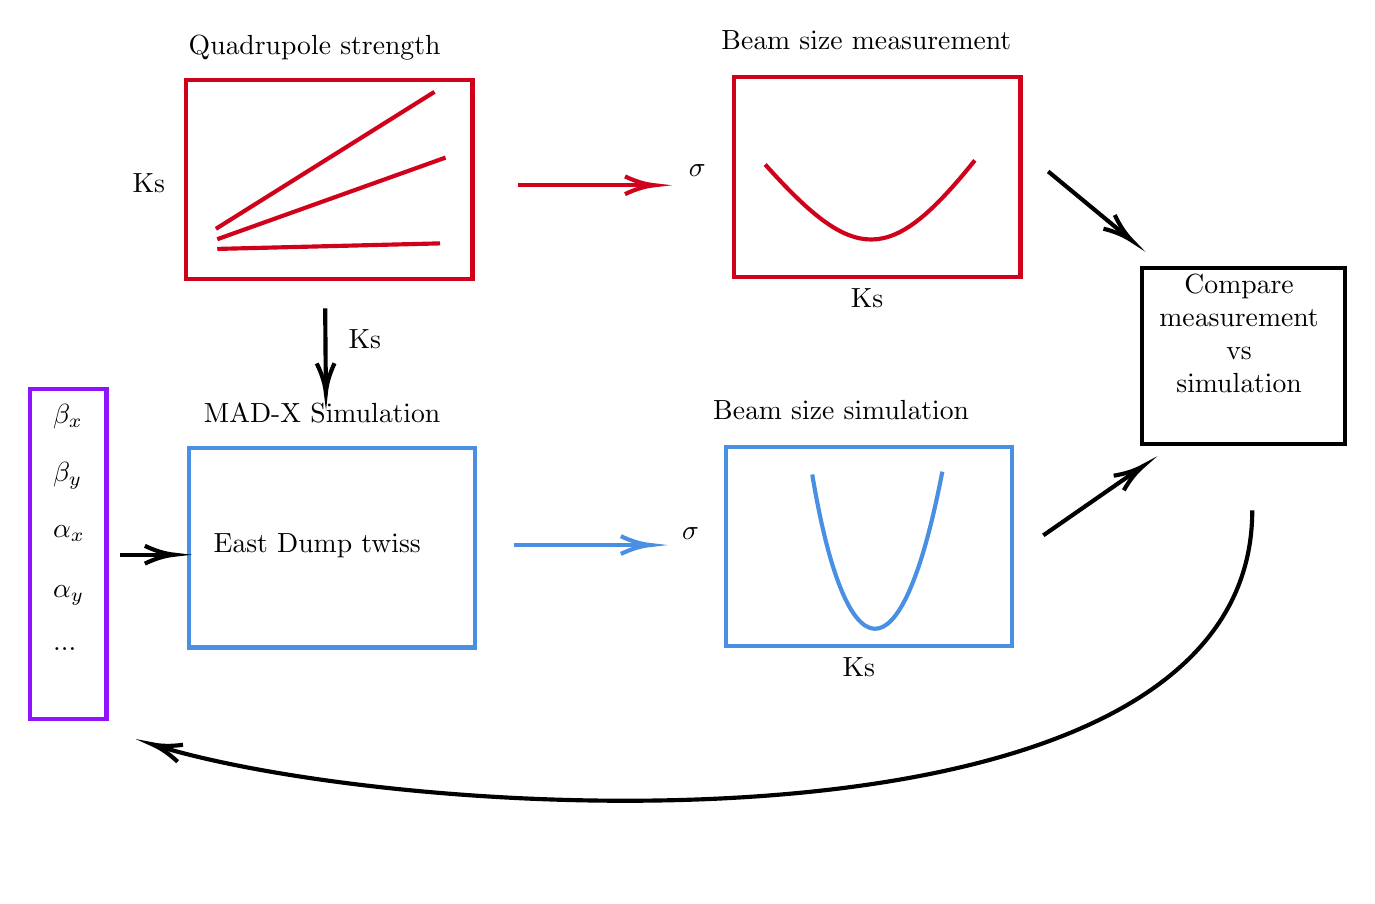
\begin{tikzpicture}[x=0.75pt,y=0.75pt,yscale=-1,xscale=1]
%uncomment if require: \path (0,480); %set diagram left start at 0, and has height of 480

%Shape: Rectangle [id:dp4246347329167801] 
\draw  [color={rgb, 255:red, 208; green, 2; blue, 27 }  ,draw opacity=1 ][line width=1.5]  (362.67,99.33) -- (500.67,99.33) -- (500.67,195.33) -- (362.67,195.33) -- cycle ;
%Curve Lines [id:da9888709896390471] 
\draw [color={rgb, 255:red, 208; green, 2; blue, 27 }  ,draw opacity=1 ][line width=1.5]    (377.67,141.33) .. controls (420.67,189.33) and (437.67,190.33) .. (478.67,139.33) ;
%Shape: Rectangle [id:dp49952149002749646] 
\draw  [color={rgb, 255:red, 208; green, 2; blue, 27 }  ,draw opacity=1 ][line width=1.5]  (98.67,100.67) -- (236.67,100.67) -- (236.67,196.67) -- (98.67,196.67) -- cycle ;
%Straight Lines [id:da9425896029593615] 
\draw [color={rgb, 255:red, 208; green, 2; blue, 27 }  ,draw opacity=1 ][line width=1.5]    (113,172.33) -- (218.33,106.33) ;
%Straight Lines [id:da0776144392613658] 
\draw [color={rgb, 255:red, 208; green, 2; blue, 27 }  ,draw opacity=1 ][line width=1.5]    (113.67,177.33) -- (223.67,138) ;
%Straight Lines [id:da02037742317127811] 
\draw [color={rgb, 255:red, 208; green, 2; blue, 27 }  ,draw opacity=1 ][line width=1.5]    (113.67,182) -- (221,179.33) ;
%Straight Lines [id:da070053405995959] 
\draw [color={rgb, 255:red, 208; green, 2; blue, 27 }  ,draw opacity=1 ][line width=1.5]    (258.67,151.33) -- (321.33,151.33) ;
\draw [shift={(324.33,151.33)}, rotate = 180] [color={rgb, 255:red, 208; green, 2; blue, 27 }  ,draw opacity=1 ][line width=1.5]    (14.21,-4.28) .. controls (9.04,-1.82) and (4.3,-0.39) .. (0,0) .. controls (4.3,0.39) and (9.04,1.82) .. (14.21,4.28)   ;
%Shape: Rectangle [id:dp944364271889234] 
\draw  [color={rgb, 255:red, 144; green, 19; blue, 254 }  ,draw opacity=1 ][line width=1.5]  (23.33,249.33) -- (60.33,249.33) -- (60.33,408.67) -- (23.33,408.67) -- cycle ;
%Straight Lines [id:da8395245156263087] 
\draw [color={rgb, 255:red, 0; green, 0; blue, 0 }  ,draw opacity=1 ][line width=1.5]    (165.67,210.67) -- (165.98,248.33) ;
\draw [shift={(166,251.33)}, rotate = 269.53] [color={rgb, 255:red, 0; green, 0; blue, 0 }  ,draw opacity=1 ][line width=1.5]    (14.21,-4.28) .. controls (9.04,-1.82) and (4.3,-0.39) .. (0,0) .. controls (4.3,0.39) and (9.04,1.82) .. (14.21,4.28)   ;
%Shape: Rectangle [id:dp4855606702968256] 
\draw  [color={rgb, 255:red, 74; green, 144; blue, 226 }  ,draw opacity=1 ][line width=1.5]  (100,278) -- (238,278) -- (238,374) -- (100,374) -- cycle ;
%Straight Lines [id:da7022632349262303] 
\draw [line width=1.5]    (66.67,329.33) -- (90,329.33) ;
\draw [shift={(93,329.33)}, rotate = 180] [color={rgb, 255:red, 0; green, 0; blue, 0 }  ][line width=1.5]    (14.21,-4.28) .. controls (9.04,-1.82) and (4.3,-0.39) .. (0,0) .. controls (4.3,0.39) and (9.04,1.82) .. (14.21,4.28)   ;
%Straight Lines [id:da3968621494939437] 
\draw [color={rgb, 255:red, 74; green, 144; blue, 226 }  ,draw opacity=1 ][line width=1.5]    (256.67,324.67) -- (319.33,324.67) ;
\draw [shift={(322.33,324.67)}, rotate = 180] [color={rgb, 255:red, 74; green, 144; blue, 226 }  ,draw opacity=1 ][line width=1.5]    (14.21,-4.28) .. controls (9.04,-1.82) and (4.3,-0.39) .. (0,0) .. controls (4.3,0.39) and (9.04,1.82) .. (14.21,4.28)   ;
%Shape: Rectangle [id:dp4118518001915987] 
\draw  [color={rgb, 255:red, 74; green, 144; blue, 226 }  ,draw opacity=1 ][line width=1.5]  (358.67,277.33) -- (496.67,277.33) -- (496.67,373.33) -- (358.67,373.33) -- cycle ;
%Curve Lines [id:da2553267141266382] 
\draw [color={rgb, 255:red, 74; green, 144; blue, 226 }  ,draw opacity=1 ][line width=1.5]    (400.33,290.67) .. controls (416.33,386.67) and (443,393.33) .. (463,289.33) ;
%Shape: Rectangle [id:dp8890861260646525] 
\draw  [line width=1.5]  (559.33,191.33) -- (657,191.33) -- (657,276) -- (559.33,276) -- cycle ;
%Curve Lines [id:da18599849782409872] 
\draw [line width=1.5]    (612.33,308) .. controls (612.33,483.12) and (203.78,458.25) .. (84.12,421.23) ;
\draw [shift={(82.33,420.67)}, rotate = 17.65] [color={rgb, 255:red, 0; green, 0; blue, 0 }  ][line width=1.5]    (14.21,-4.28) .. controls (9.04,-1.82) and (4.3,-0.39) .. (0,0) .. controls (4.3,0.39) and (9.04,1.82) .. (14.21,4.28)   ;
%Straight Lines [id:da014820791284121837] 
\draw [line width=1.5]    (511.67,320) -- (557.2,288.38) ;
\draw [shift={(559.67,286.67)}, rotate = 145.22] [color={rgb, 255:red, 0; green, 0; blue, 0 }  ][line width=1.5]    (14.21,-4.28) .. controls (9.04,-1.82) and (4.3,-0.39) .. (0,0) .. controls (4.3,0.39) and (9.04,1.82) .. (14.21,4.28)   ;
%Straight Lines [id:da7493093229877397] 
\draw [line width=1.5]    (514,144.67) -- (552.02,176.09) ;
\draw [shift={(554.33,178)}, rotate = 219.57] [color={rgb, 255:red, 0; green, 0; blue, 0 }  ][line width=1.5]    (14.21,-4.28) .. controls (9.04,-1.82) and (4.3,-0.39) .. (0,0) .. controls (4.3,0.39) and (9.04,1.82) .. (14.21,4.28)   ;

% Text Node
\draw (417.67,199.83) node [anchor=north west][inner sep=0.75pt]   [align=left] {Ks};
% Text Node
\draw (339.67,140.33) node [anchor=north west][inner sep=0.75pt]   [align=left] {$\displaystyle \sigma $};
% Text Node
\draw (71.67,144.5) node [anchor=north west][inner sep=0.75pt]   [align=left] {Ks};
% Text Node
\draw (98.67,77.67) node [anchor=north west][inner sep=0.75pt]   [align=left] {Quadrupole strength};
% Text Node
\draw (355.33,75.67) node [anchor=north west][inner sep=0.75pt]   [align=left] {Beam size measurement};
% Text Node
\draw (33.33,255.4) node [anchor=north west][inner sep=0.75pt]    {$\beta _{x}$};
% Text Node
\draw (33.33,283.4) node [anchor=north west][inner sep=0.75pt]    {$\beta _{y}$};
% Text Node
\draw (33.33,314.07) node [anchor=north west][inner sep=0.75pt]    {$\alpha _{x}$};
% Text Node
\draw (33.33,342.73) node [anchor=north west][inner sep=0.75pt]    {$\alpha _{y}$};
% Text Node
\draw (33.33,372.73) node [anchor=north west][inner sep=0.75pt]    {$...$};
% Text Node
\draw (106,255) node [anchor=north west][inner sep=0.75pt]   [align=left] {MAD-X Simulation};
% Text Node
\draw (110.67,317.67) node [anchor=north west][inner sep=0.75pt]   [align=left] {East Dump twiss};
% Text Node
\draw (413.67,377.83) node [anchor=north west][inner sep=0.75pt]   [align=left] {Ks};
% Text Node
\draw (336.33,315) node [anchor=north west][inner sep=0.75pt]   [align=left] {$\displaystyle \sigma $};
% Text Node
\draw (351.33,253.67) node [anchor=north west][inner sep=0.75pt]   [align=left] {Beam size simulation};
% Text Node
\draw (561.33,193) node [anchor=north west][inner sep=0.75pt]   [align=left] {\begin{minipage}[lt]{65.09pt}\setlength\topsep{0pt}
\begin{center}
Compare\\measurement\\vs\\simulation
\end{center}

\end{minipage}};
% Text Node
\draw (175.67,219.83) node [anchor=north west][inner sep=0.75pt]   [align=left] {Ks};

\end{tikzpicture}
}
    \caption{Initial condition diagram}
    \label{fig:initial_condition_diagram}
\end{figure}

\subsubsection{Result of the optimization}

Figure \ref{fig:combined_measurements} shows the four quadrupole scan measurement used to determine the initial conditions as well as the MAD-X predictions using the initial conditions that it converged on. The right side of the figure shows the combination of current applied where each measurement was repeated five times.
\\

\begin{figure}[htbp]
\centering
\includegraphics[width=0.7\textwidth]{03_Empirical_Measurements/images/combine_quadrupole_scan_east_dump.png}
\caption{Quadrupole scan to the East Dump compared to the MAD-X prediction using the inital conditions found through optimization. The x-scale on the left side of the figure is labeled K1 QFN01 to present the data on a plot but the three quadrupole were modified during the scan.}
\label{fig:combined_measurements}
\end{figure}

It is expected that the measurement and simulation with the East Dump will be close as they were optimized on and the East Dump line is a short line with only a few quadrupole. Of particular interested would be to assess how accurate the MAD-X model is through the main lines in the East Area where no measurement. Figure \ref{fig:comparison_btv96} show how the model predicts the minimums and maximums in beam size at BTV96 located in CHARM at the end of the T8 line. The absolute beam size measurement is however underestimated. An offset is observed in both planes where the measurements are slightly larger. This emittance mismatch can be explained by the large amount of air present in the transfer line in particular in the IRRAD experimental area which would effectively increase the emittances. Nevertheless, this first iteration of the method of using a parallel and short transfer line (East Dump 35 m) to predict the T8 line (135 m) with five additional quadrupoles and dipole can be used to make informed decisions about the optics of the line.

\begin{figure}[htbp]
\centering
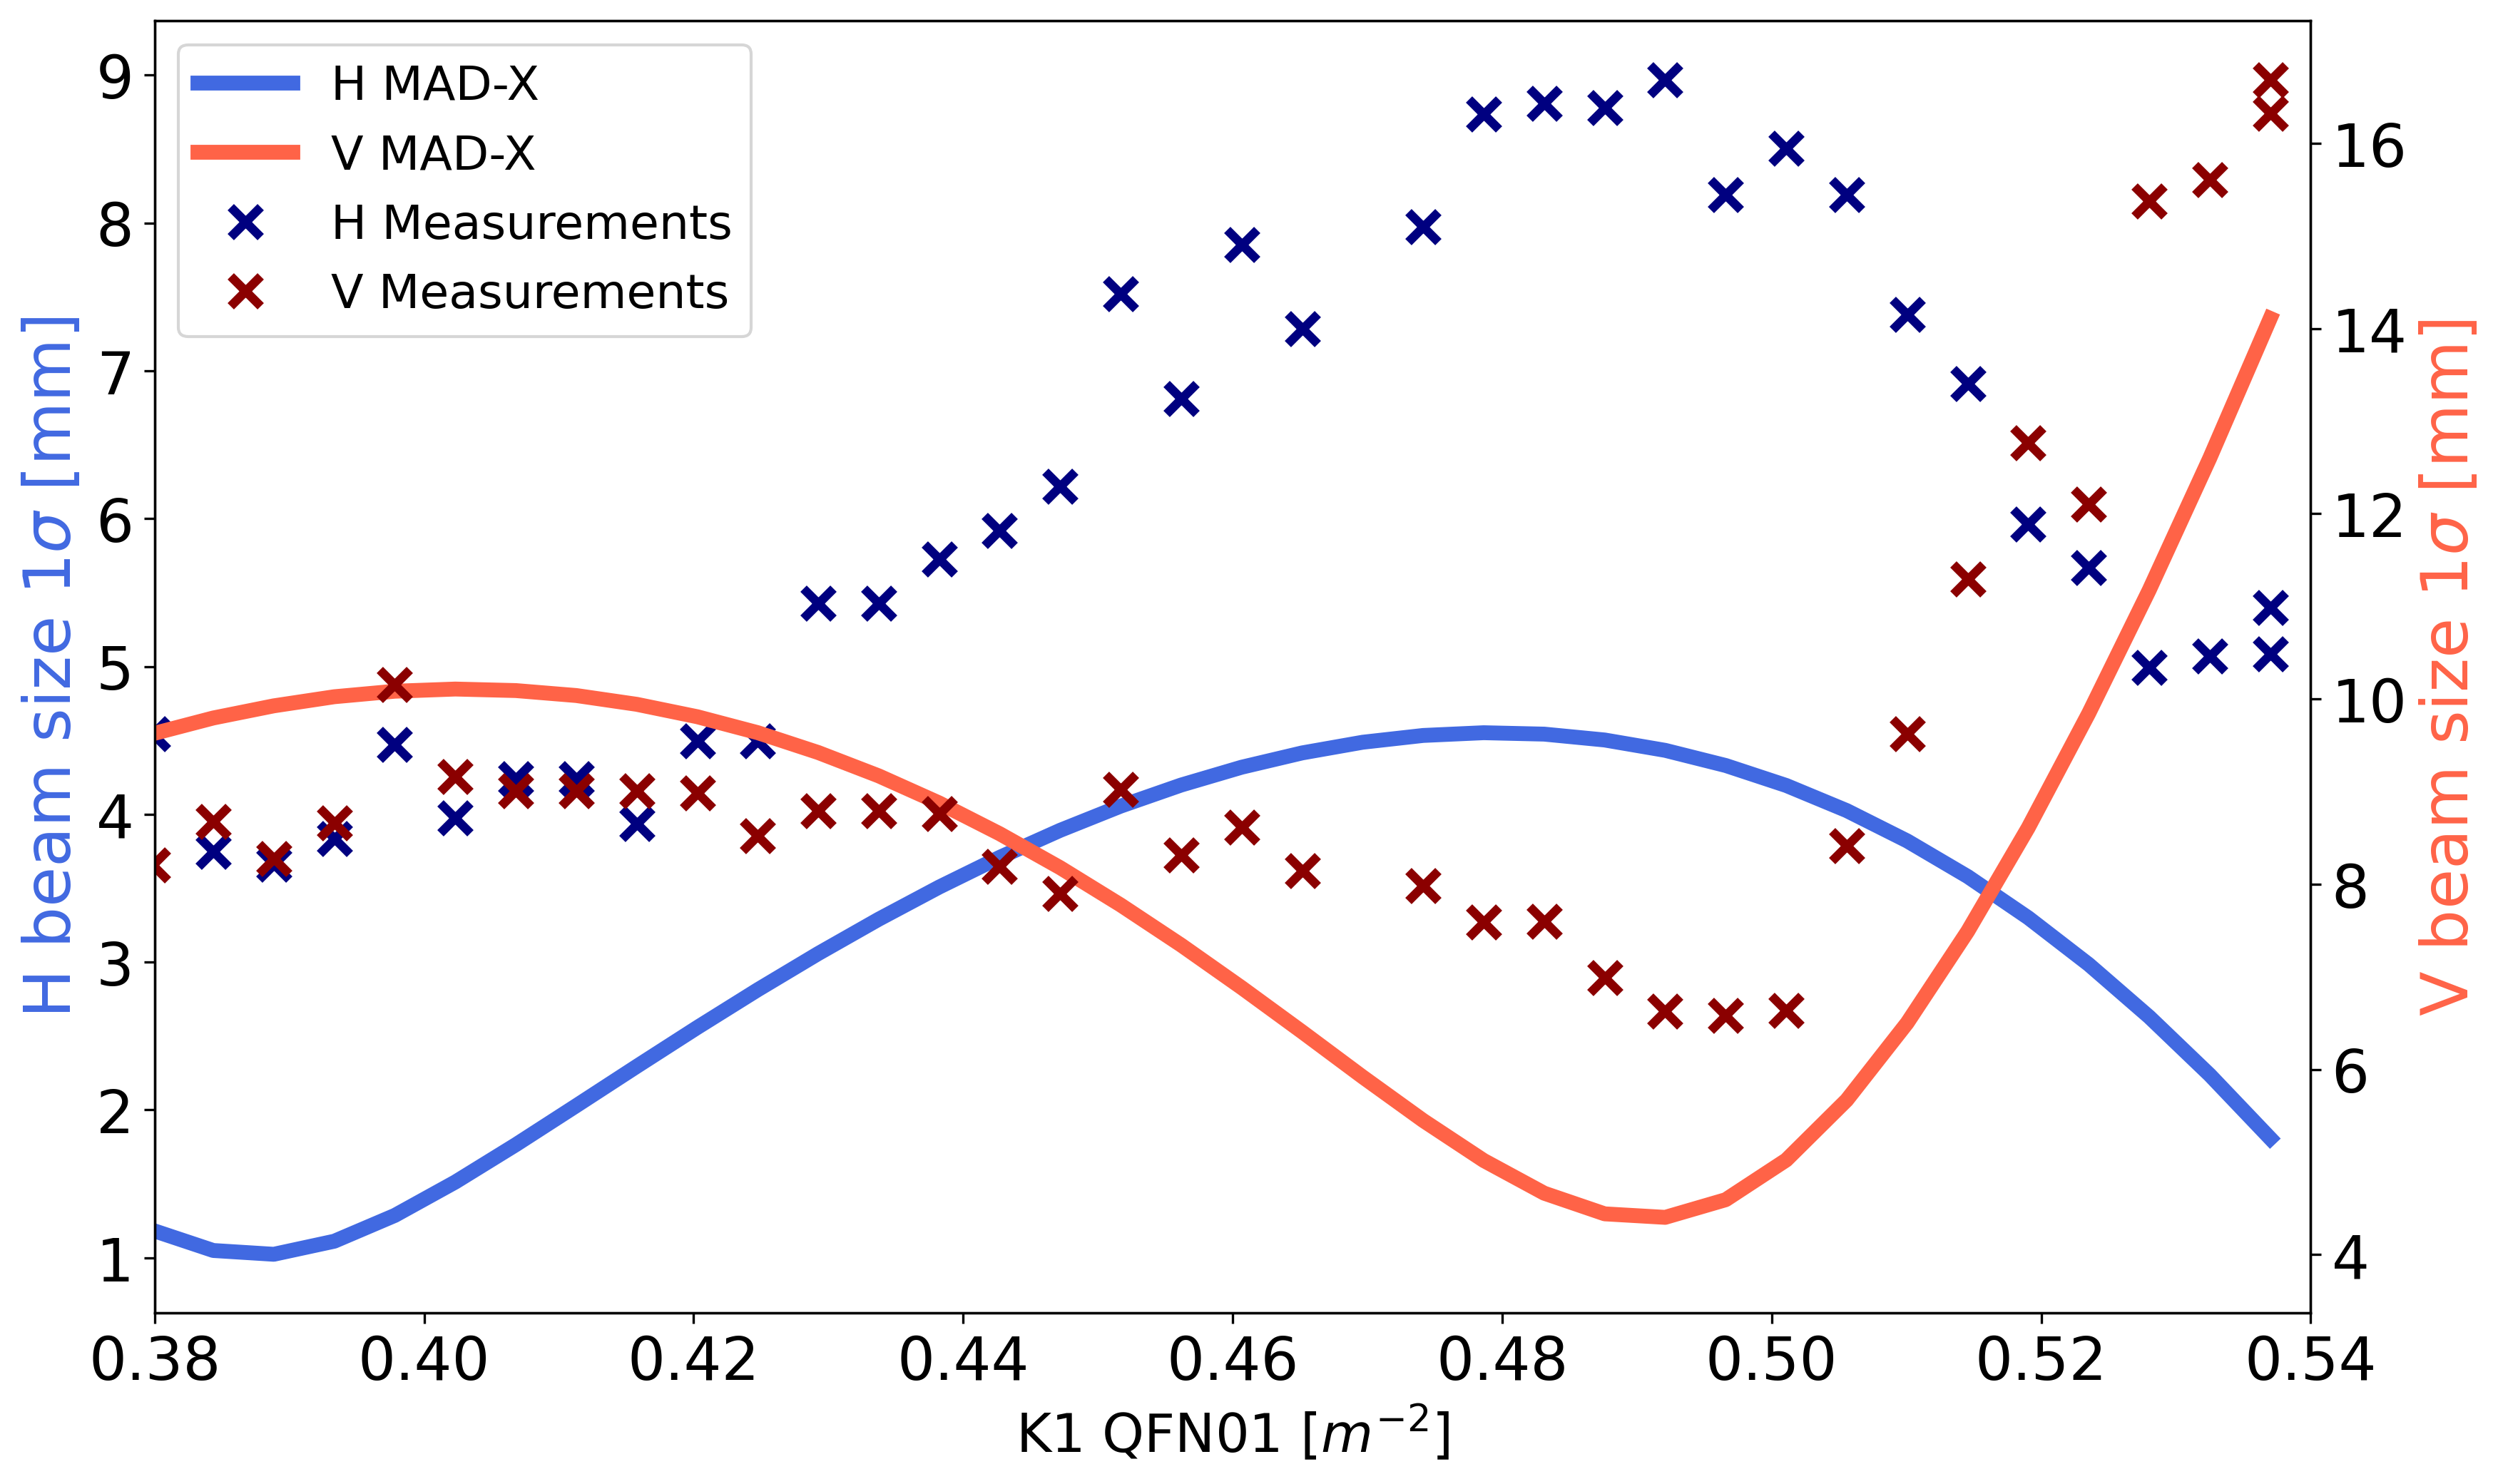
\includegraphics[width=0.7\textwidth]{03_Empirical_Measurements/images/east_quad_scan_df_meas_btv96.pickle.png}
\caption{Comparison between MAD-X model and beam size measurement in the CHARM area.}
\label{fig:comparison_btv96}
\end{figure}


\newpage
\subsubsection{Initial beam parameters of the East Area slow extracted beam}

The initial parameters located upstream of the first quadrupole of the transfer line (Q74) are presented in Table \ref{table:beam_parameters_1} and \ref{table:beam_parameters_2}.


\begin{table}[htbp]
\centering
\caption{Initial Beam Parameters - Part 1}
\label{table:beam_parameters_1}
\begin{tabular}{|c|c|c|c|c|c|c|c|}
\hline
$\beta_{x}$ [m] & $\beta_{y}$ [m] & $\alpha_{x}$ & $\alpha_{y}$ & $D_{x}$ [m] & $D_{y}$ [m] & $D^{'}_{x}$[mrad] & $D^{'}_{y}$[mrad] \\
\hline
154.1 & 5.22 & -36.9 & 0.25 & 0.13 & 0.0 & 0.02 & 0.0 \\
\hline
\end{tabular}
\end{table}

\begin{table}[htbp]
\centering
\caption{Initial Beam Parameters - Part 2}
\label{table:beam_parameters_2}
\begin{tabular}{|c|c|c|}
\hline
$e_{xn}$ [m] & $e_{yn}$ [m] & $\frac{\Delta p}{p}$ \\
\hline
7.64e-06 & 3.53e-06 & 6.79e-4 \\
\hline
\end{tabular}
\end{table}


\subsection{EAST Area T8 optics 2023}

% For this part, you should describe:
% The reason for implementing new optics to the EAST area.
% The method used for this implementation and the considerations taken into account.
% The result of this new implementation, emphasizing the alignment with the initial parameters.

\subsubsection{Reasons for implementing new optics to the East Area}

The optics used during 2021 and 2022 in the T8 line needed to be modified as a large "tail", see Fig. \ref{fig:tail_irrad} was present in the horizontal plane which isn't ideal for the irradiation operations in IRRAD.
\\

\begin{figure}[H]
\centering
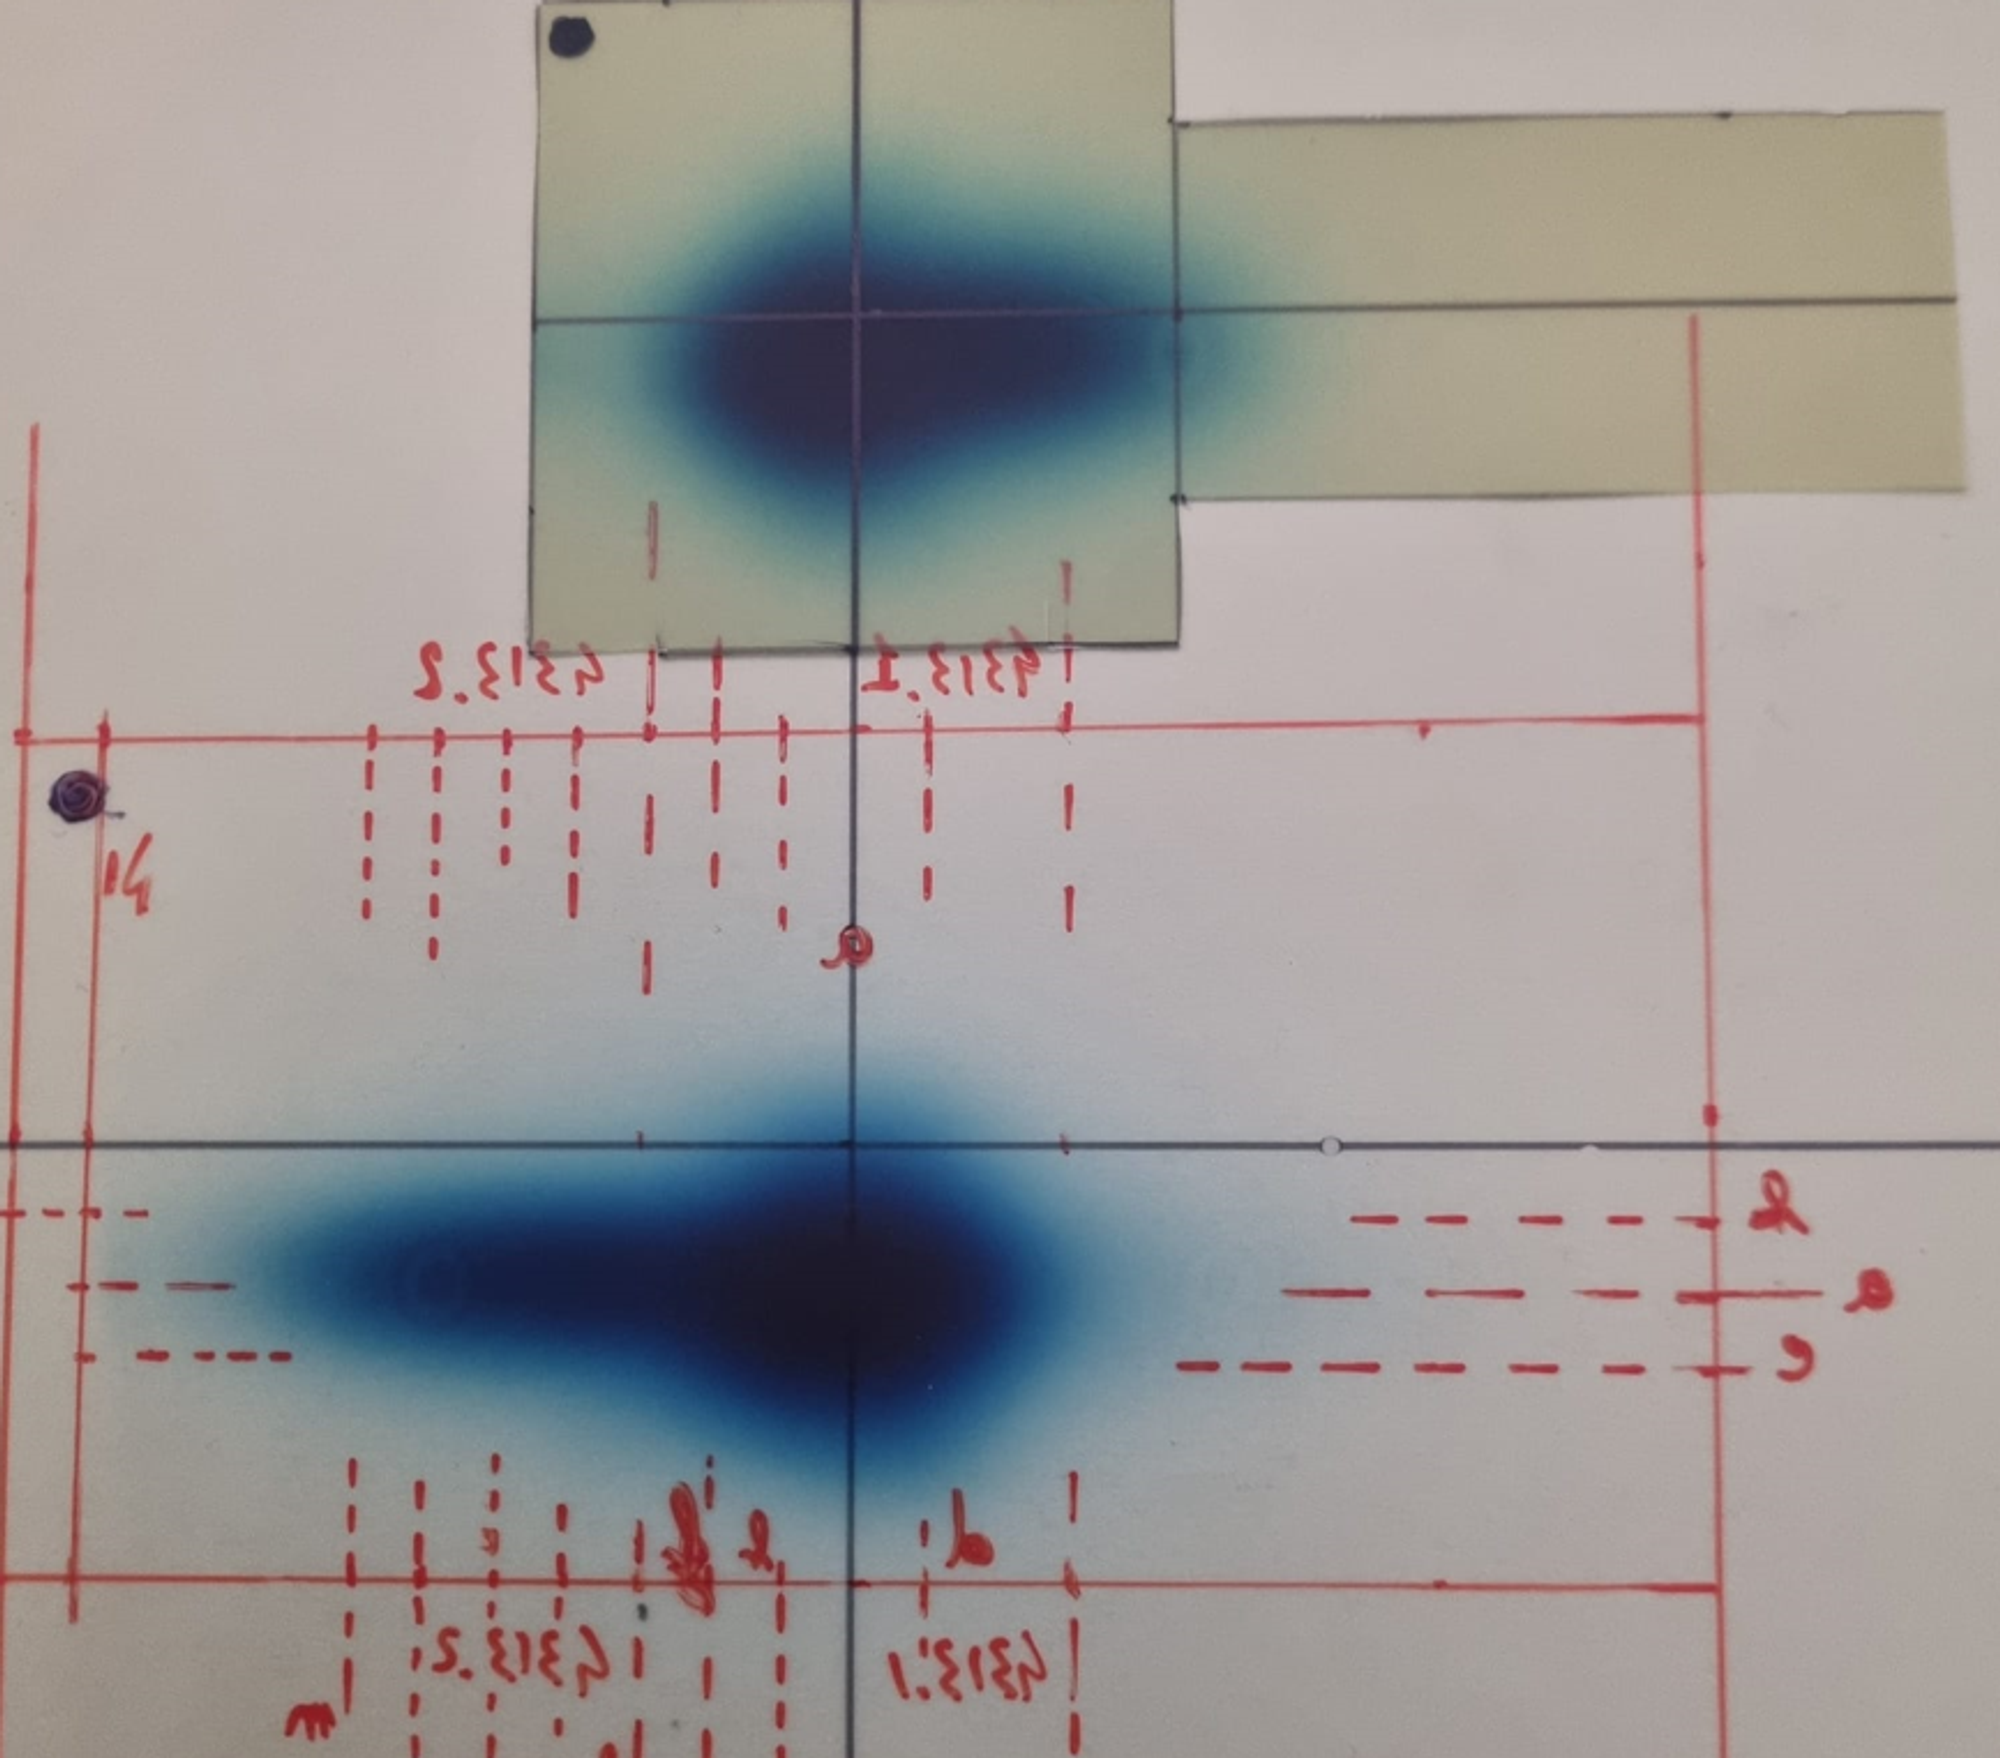
\includegraphics[width=0.6\textwidth]{03_Empirical_Measurements/images/tail_irrad.png}
\caption{GAFchromic film in IRRAD showing the "tail" before (bottom) and after (top) using the horizontal dipole corrector.}
\label{fig:tail_irrad}
\end{figure}

The tail is caused by the natural sweep due to an non-constant optics that starts in the PS ring and that propagate (and becomes larger) in the transfer line. This is particularly observed and unwanted in IRRAD that need symmetric round and parallel beams across there four irradiation stations. Initial hypothesis if dispersion in this region could cause asymmetric beam. While it is true that the dispersion is non-zero and non-linear at the IRRAD irradiation stations which could produce a tail, see Fig. \ref{fig:nonlinear_dispersion}, PTC simulation show, see Fig. \ref{fig:PTC_dispersion}, that to reproducing these tails require an offset in momentum of 3\% which is orders of magnitude away from the real beam momentum spread which is closer to 0.03\% $\frac{\Delta p}{p}$.

\begin{figure}[htbp]
\centering
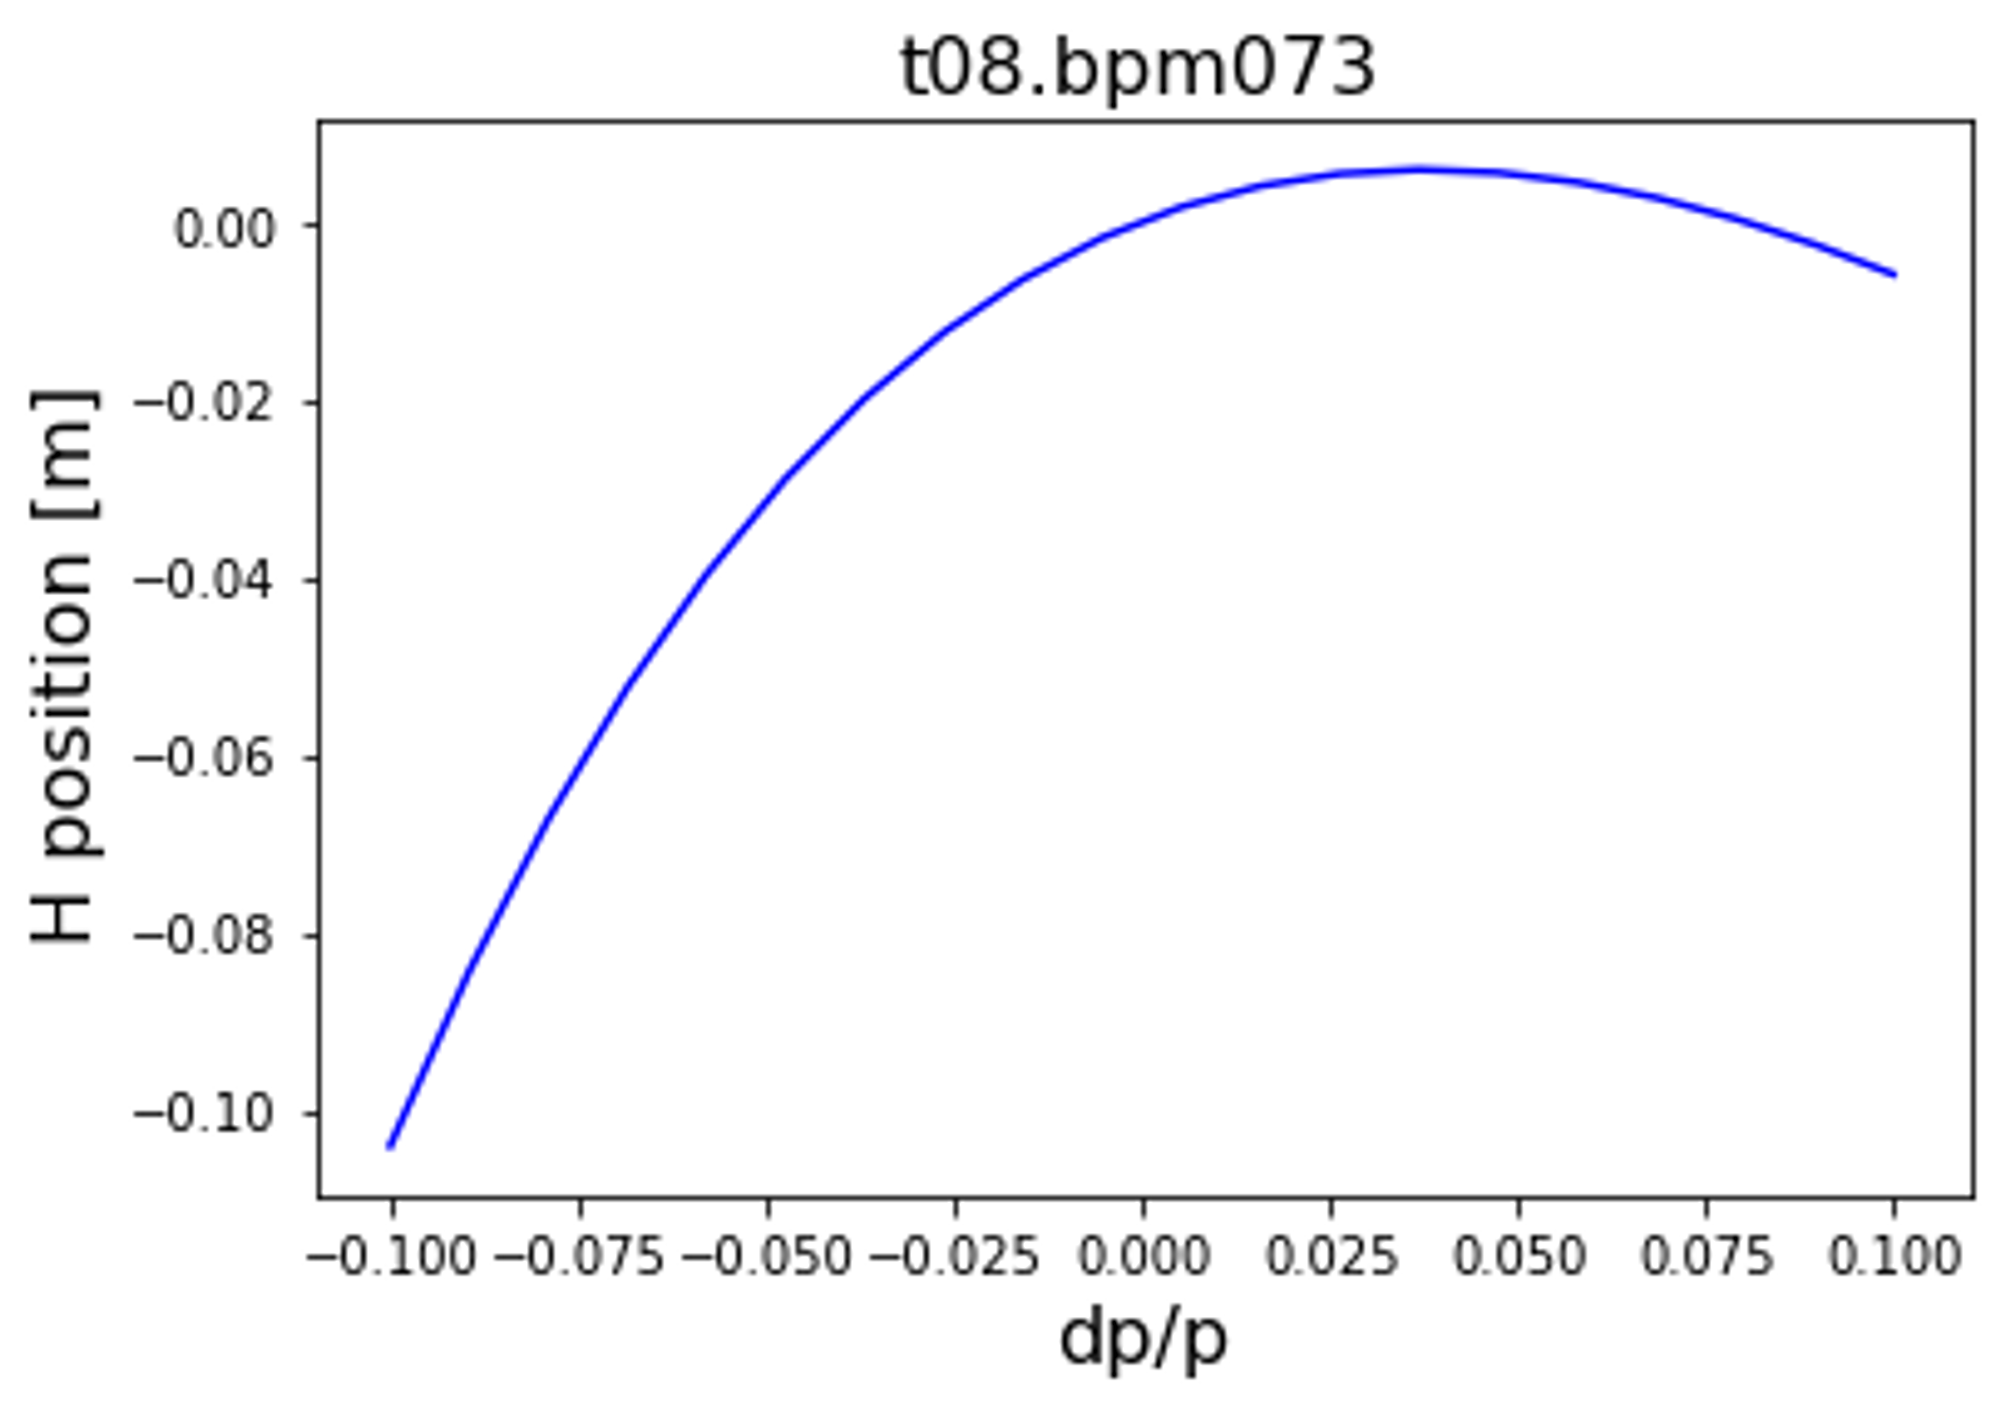
\includegraphics[width=0.5\textwidth]{03_Empirical_Measurements/images/nonlinear_dispersion.png}
\caption{Non-linear dispersion at IRRAD BPM1.}
\label{fig:nonlinear_dispersion}
\end{figure}

\begin{figure}[htbp]
\centering
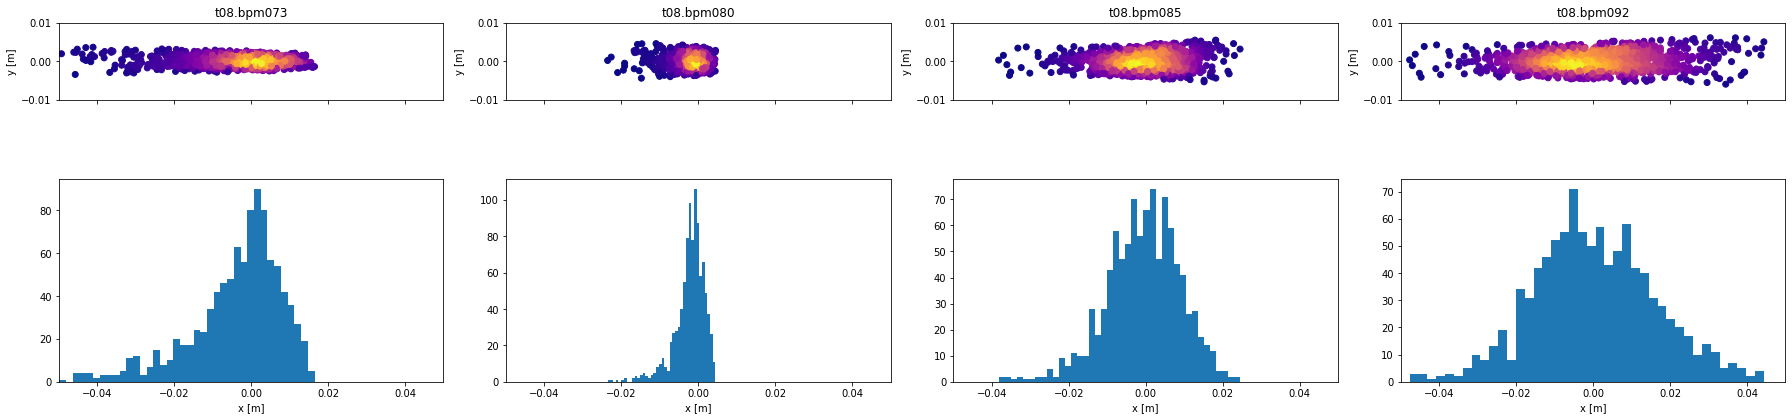
\includegraphics[width=1.0\textwidth]{03_Empirical_Measurements/images/dispersion_3percent_dpp.png}
\caption{PTC simulation of the beam distribution in real space at the IRRAD BPMs location.}
\label{fig:PTC_dispersion}
\end{figure}

Knowing that the tail was only produced by the sweep, a linear ramp on a horizontal corrector magnet was set-up to cancel it. This indeed lowered the amount of tail but also changed it's side which means we crossed a focal point. However as there are no instrumentation capable of producing multiple acquisitions during a single spill at the irradiation point it is difficult to cancel the tail through this method.

\subsubsection{Methodology for Implementing New Optics and Key Considerations}

The methodology for implementing the new optics was guided by the requisites and constraint from the IRRAD team, using the MAD-X model of the line in tandem with an optimiser. The key specifications revolved around achieving an 13mm $\times$ 13.6mm full-width half-maximum (FWHM) beam, both symmetric and parallel across the four irradiation zones. A MAD-X model of the beam was used and optimized with these given constraints to produce new optics using the eight quadrupoles available in F61 and T8 and the initial conditions from Table \ref{table:beam_parameters_1} and \ref{table:beam_parameters_2}.
\\

Fast iterations were made possible by using a script that uploads the newly produces optics to the CCC computers, followed by setting them using Py-Japc. Iterations were necessary due to the observed divergence between the model and the real-world measurements; particularly, the model does not perfectly predict the absolute beam size, notably in the CHARM area, the second irradiation area and the most downstream part of the transfer line.
\\

As a result, the optics optimizer didn't actually use the specified constrained but rather values close to it so that the actually beam would match the specifications. Additionally, it was noticed that large changes to the most upstream quadrupoles (Q74L, specifically, being close to the stray fields) degraded heavily the beam. To circumvent this issue, only minor modifications were applied to these upstream quadrupoles --- within a few percent, whereas the quadrupoles in closer proximity to the irradiation area were permitted a full range of strength variation.
\\

This model-informed iterative approach considerably expedited the process, enabling the implementation of new optics within a few hours. The incorporation of an air scattering model may further enhance the accuracy and precision of the model, facilitating changes in the optics even further.


\subsubsection{Results of the new optics implementation}

After a few iterations, a satisfactory new optics was selected for the T8 line. Table \ref{table:New optics quadrupole strenghts} presents the quadrupole strengths of the optics implemented in April 2023 for the T8 line.

\begin{table}[htbp]
    \centering
    \caption{Quadrupole Strengths}
    \begin{tabular}{cc}
        \hline
        Quadrupole & K1 [$\text{m}^{-2}$] \\
        \hline
        kQFN1 & 0.49169 \\
        kQDN2 & -0.18725 \\
        kQFN3 & 0.2142 \\
        kQDN4 & -0.07838 \\
        kQFN5 & 0.1877 \\
        kQDN6 & -0.1922 \\
        kQDN7 & -0.07342 \\
        kQFN8 & 0.06299 \\
        \hline
    \end{tabular}
    \label{table:New optics quadrupole strenghts}
\end{table}

The comparison between the simulation and experimental measurements is depicted in Figure \ref{fig:IRRAD_new_optics_sim_meas_comparison}. The blue curve denotes the simulation results for the one sigma horizontal beam size, while the red curve represents the vertical beam size. Markers have been added at the locations of the IRRAD BPMs to show beam size measurements averaged over a few hours (09:41 to 12:00 20/04/2023). A notable degree of conformity is observed in both planes, with a markedly good agreement in the vertical plane. The error bars, symbolizing the standard deviation for the beam size measurements, appear larger in the horizontal plane.

\begin{figure}[htbp]
\centering
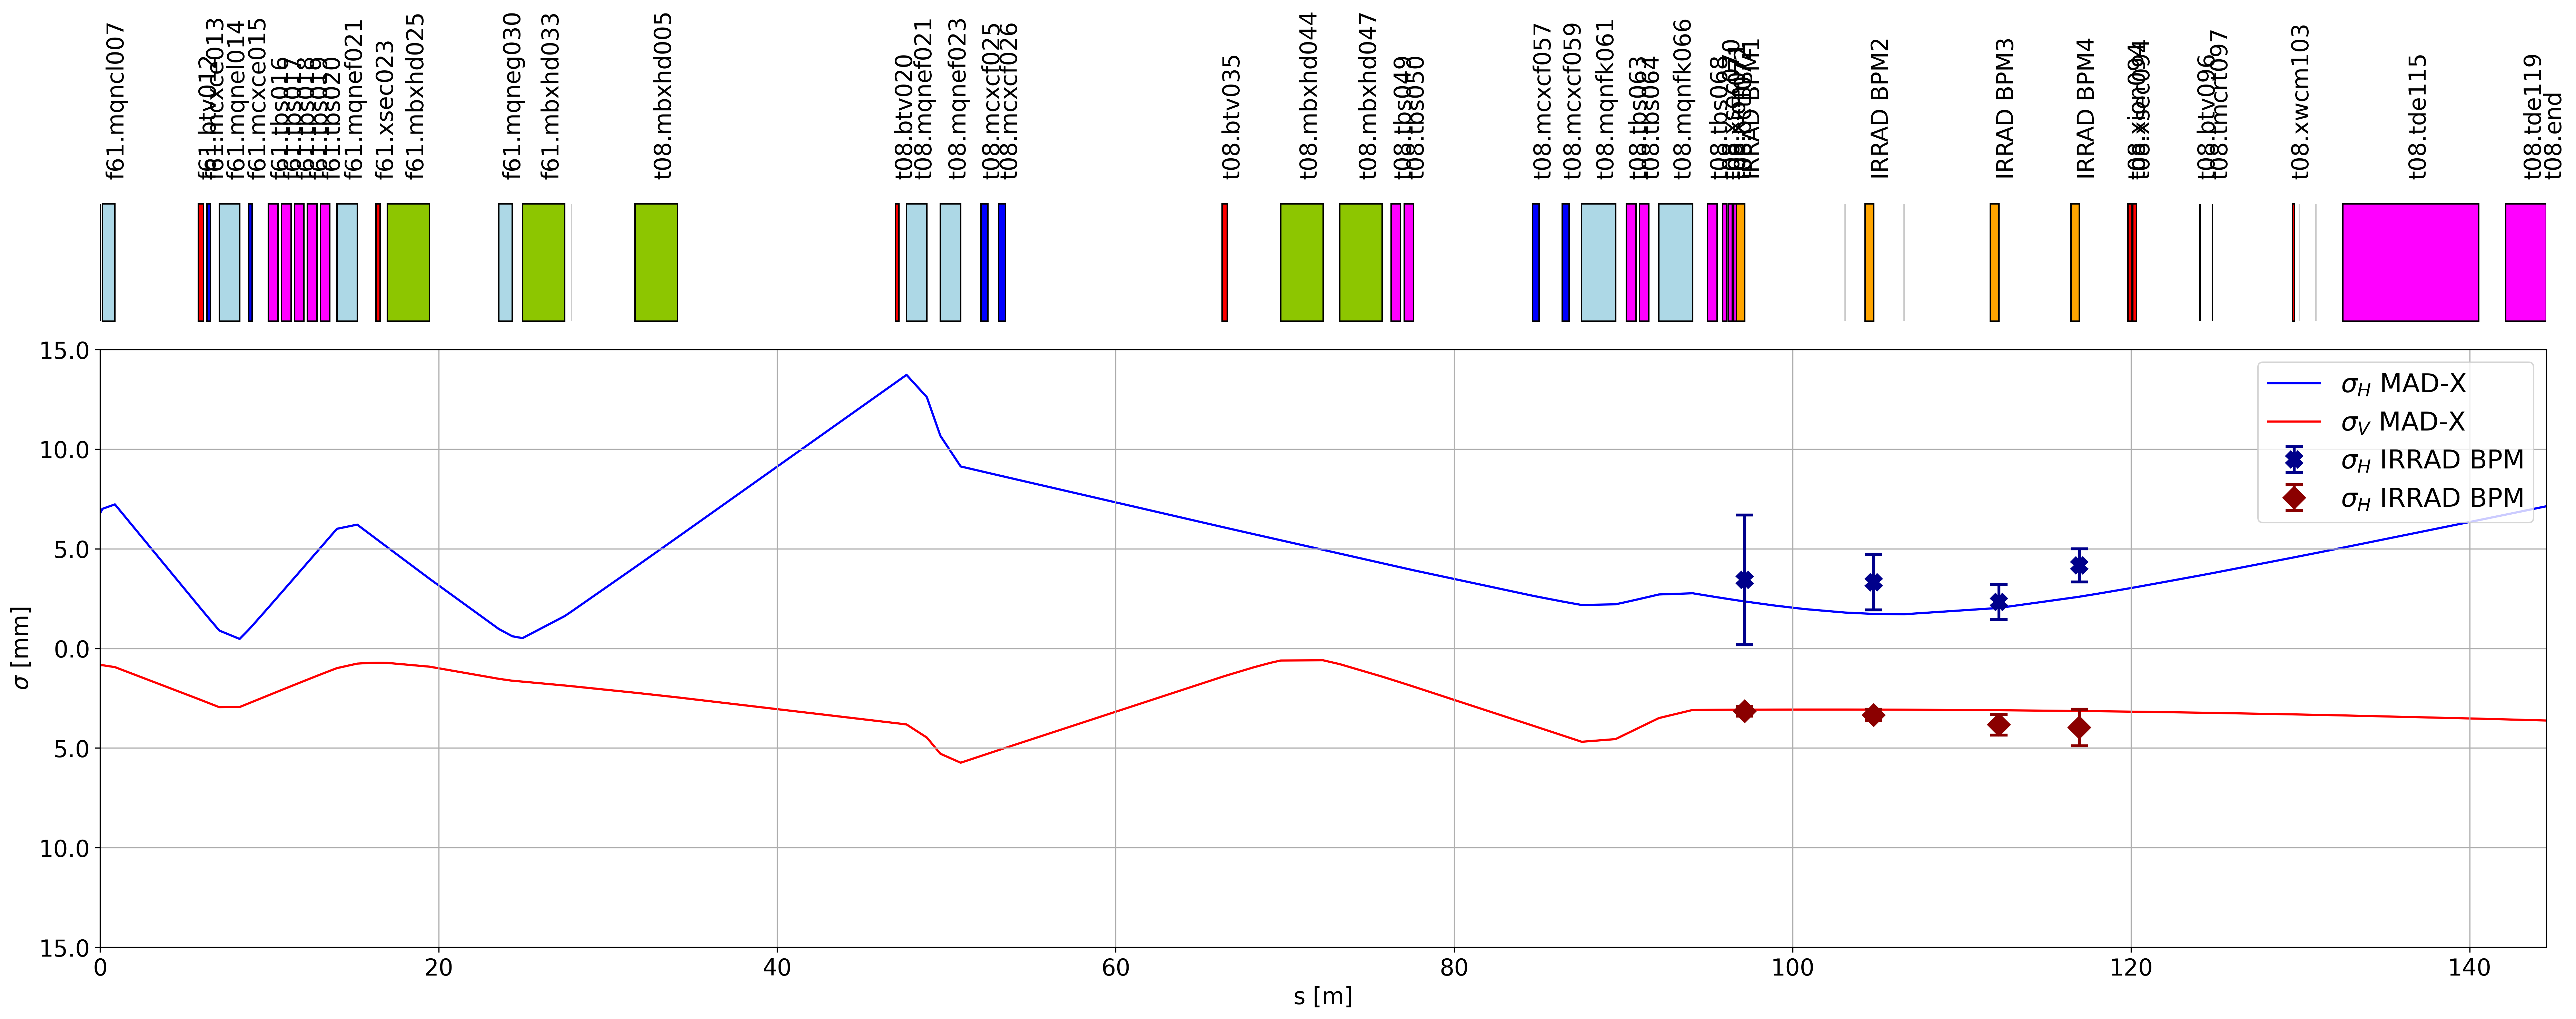
\includegraphics[width=1.0\textwidth]{03_Empirical_Measurements/images/t8_optics_with_measurement_zoom.png}
\caption{Comparison between the MAD-X model of the T8 line and the measurements at the IRRAD BPMs.}
\label{fig:IRRAD_new_optics_sim_meas_comparison}
\end{figure}

Figure \ref{fig:error_irrad_sim} shows the difference between the measurements and the simulation. It appears that the simulation under estimates the real beam size in a constant manner. In the horizontal plane the disagreement comes close to -50\% for BPM2. In the vertical plane the agreement is better. One however observes a trend in increase in disagreement which might be associated with emittance blowup due to air scattering.

\begin{figure}[htbp]
\centering
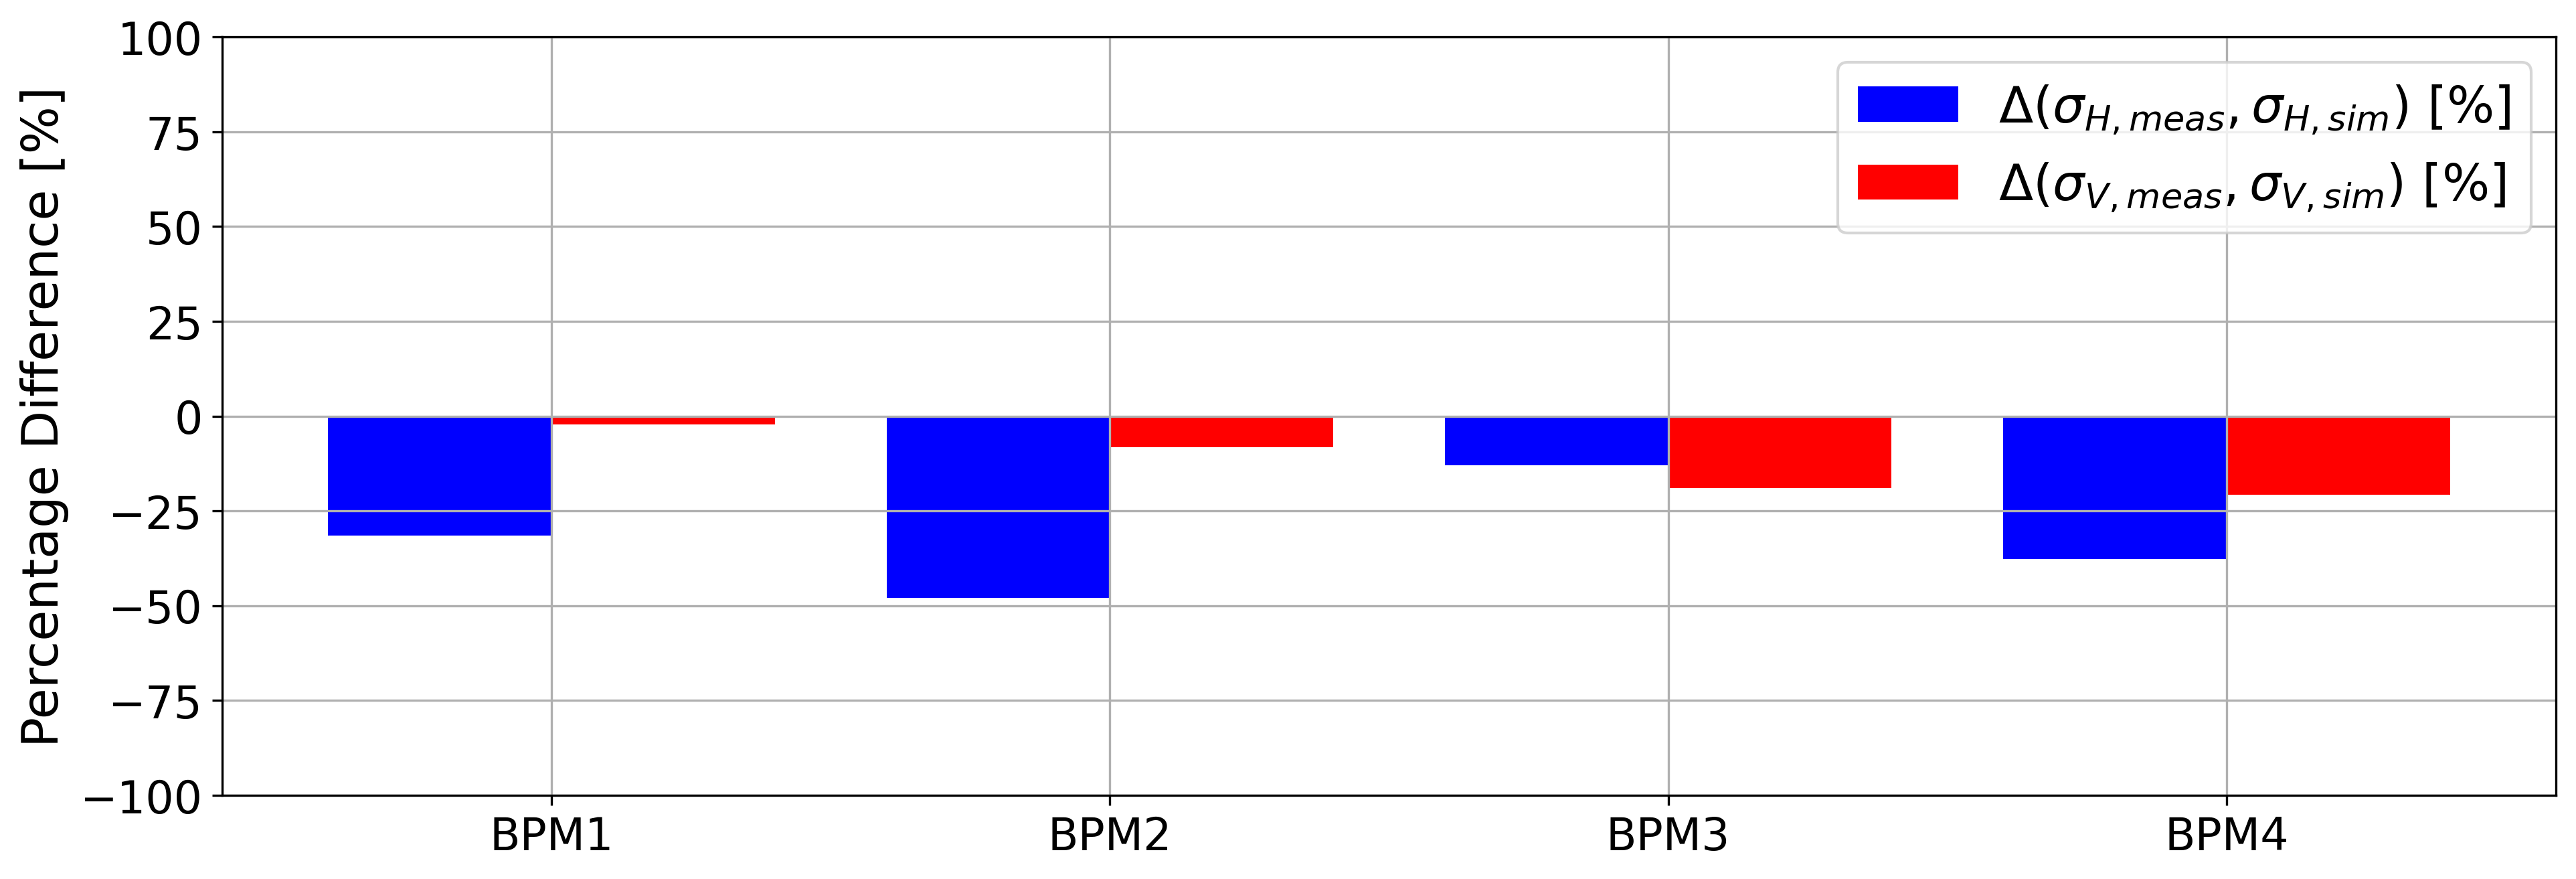
\includegraphics[width=0.9\textwidth]{03_Empirical_Measurements/images/percentage_diff_btw_sigma_meas_and_sim.png}
\caption{Percentage difference between beam size measurement median and simulation}
\label{fig:error_irrad_sim}
\end{figure}

% Figure \ref{fig:irrad_bpms_new_optics} shows the signal on the IRRAD BPMs.

% \begin{figure}[htbp]
% \centering
% 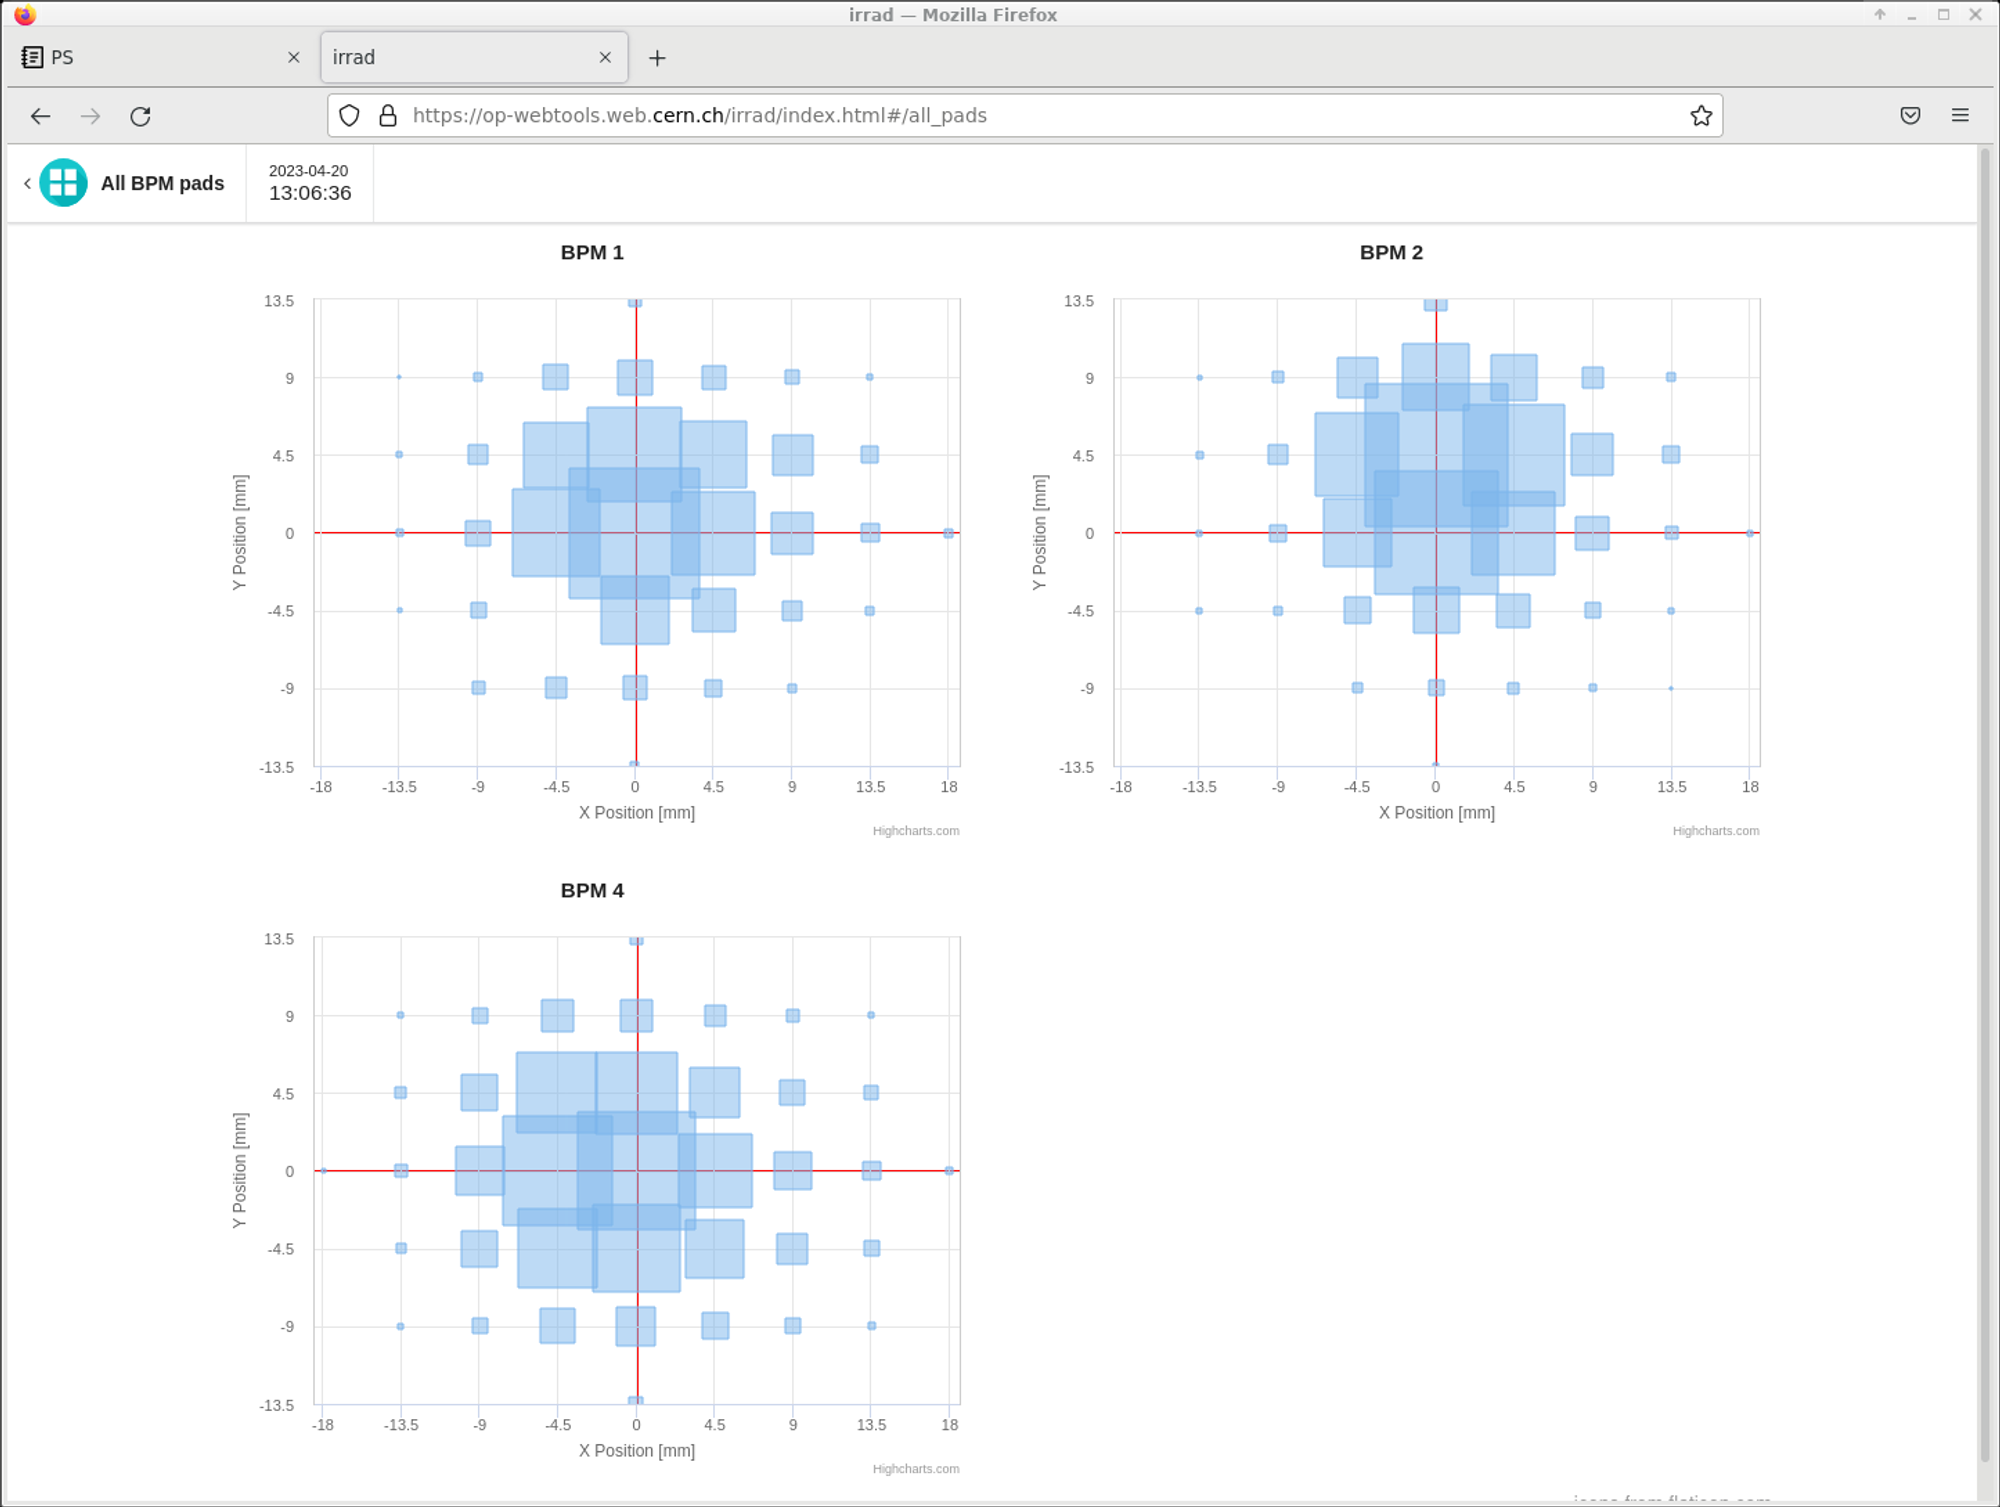
\includegraphics[width=1.0\textwidth]{03_Empirical_Measurements/images/irrad_new_optics.png}
% \caption{PTC simulation of the beam distribution in real space at the IRRAD BPMs location.}
% \label{fig:irrad_bpms_new_optics}
% \end{figure}

\subsection{Ion initial condition}

Reference to IPAC 2024 contribution.